%!TEX root = ../thesis.tex
%*******************************************************************************
%******************************* First Chapter *********************************
%*******************************************************************************

\chapter{HIV incidence estimation}\label{cha:hivbackcalc}

\graphicspath{{02_HIVBackCalc/Figs/}}

In common with many infectious disease monitoring programmes, observable data on new HIV diagnoses are not a reliable measure of the underlying incidence of infection in a population. Signals in HIV diagnosis data can be particularly misleading for a number of reasons:\ the time from infection to diagnosis varies substantially between individuals, diagnoses may be under-reported or delayed by several years, and are subject to external forces such as mass-testing campaigns and migration~\parencite{Brizzi2017-fv}.

Even with enhanced surveillance systems and widespread availability of testing, the period during which an individual may experience no symptoms (and therefore be unaware of their HIV infection) is on the order of years rather than days or months. Quantifying the incidence and prevalence of the virus in a timely way is therefore far from straightforward.

Statistical techniques which account for these time-varying factors are therefore crucial to reconstruct the underlying prevalence and incidence of HIV from available data.

\section{Aims of this chapter}

This chapter focuses on the development and application of a multi-state modelling method known as `CD4 back-calculation', which uses:\ observed numbers of HIV diagnoses over time; the distribution of CD4 counts at, or soon after, diagnosis; and information on disease progression to reconstruct the unobserved HIV incidence and estimate quarterly probabilities of HIV diagnosis~\parencite{Birrell2012-hw, Brizzi2019-yj}.

In recent years, due to increased frequency of testing and more sensitive diagnostic tests, individuals with recently acquired HIV have been at greater risk of diagnosis during the acute phase of infection. During this acute phase, the CD4 count measurements used in the HIV back-calculation model could present a misleading picture of disease progression, which may impact upon estimates. I aim to quantify the extent to which CD4 count data may incorrectly classify an individual's progression towards AIDS, using additional information on biomarkers of recent infection. I then aim to incorporate these biomarkers into the existing CD4 back-calculation method to ensure the suitability of this model in an era of more frequent testing.

During the COVID-19 pandemic, HIV testing activity was disrupted due to healthcare service reconfiguration, and HIV transmission was likely interrupted as a result of restrictions on social mixing. The effect was an abrupt change in the number of new HIV diagnoses during 2020. I aim to investigate the sensitivity of the back-calculation model to this change, and estimate if England's ambition to end HIV transmission by 2030 remains on track~\parencite{HIV_Commission2020-yy}.

\section{Background}

\subsection{HIV in the UK}

In the UK, the HIV epidemic is highly concentrated among gay, bisexual and other men who have sex with men (GBM)\nomenclature[z]{GBM}{Gay, bisexual and other men who have sex with men}, and black African populations. In 2022, HIV prevalence was estimated to exceed 7\% and 1.8\% in these groups, respectively, compared to an overall prevalence of 0.2\% among 15-to-74 year-olds in England~\parencite{Martin2023-um}.

\subsubsection{HIV prevention targets}

The UK has seen large increases in regular and repeat HIV testing in recent years, particularly among GBM who attend sexual health services (SHS)\nomenclature[z]{SHS}{Sexual health services}, and PrEP Impact Trial participants who accessed 3-monthly testing during 2017--2020~\parencite{Brown2017-yu,Brown2018-nk,PrEP_Impact_Trial2020-il}. Meanwhile, following an update to treatment guidelines in 2015, increased uptake of HIV treatment has led to a reduction in the proportion of people living with detectable levels of HIV~\parencite{Churchill2016-ol, Martin2023-um}. As a result, there is now compelling evidence of a trend towards earlier diagnosis and a decline in HIV transmission, detected first among GBM in London, and later confirmed across England~\parencite{Brown2017-yu, Brizzi2021-zl}.

In 2020, an independent commission on HIV set ambitious targets to reduce the number of new HIV infections in England to under 600 by 2025 and under 100 by 2030, the respective targets for GBM being under 250 by 2025 and under 50 by 2030~\parencite{HIV_Commission2020-yy}. This ambition to eliminate HIV as a public health threat by 2030 remains a significant one, requiring continued investment into prevention initiatives and close monitoring of trends in HIV transmission using statistical methodologies~\parencite{HIV_Commission2020-yy, Department_of_Health_and_Social_Care2019-gd}.

\subsection{Natural history of HIV infection}

The natural history of HIV infection in the absence of treatment spans several distinct phases:\ eclipse, acute, chronic, and AIDS~\parencite{Maartens2014-xd}.

The \textbf{eclipse phase} lasts around 10 days and begins immediately following HIV transmission. During this period the virus is undetectable in blood serum (also known as the `window period')~\parencite{Cohen2010-ol}.

The \textbf{acute phase}, or `seroconversion' phase, lasts around 12 weeks and in this time viruses spread from the site of infection and enter the bloodstream, a process known as viremia. This phase ends with \textbf{seroconversion}, when HIV antibodies become detectable in the blood, and some individuals may experience flu-like symptoms around this time, known as seroconversion illness~\parencite{Cohen2010-ol, Muema2020-zr}.

The \textbf{chronic} (generally asymptomatic) \textbf{phase} lasts 6-to-7 years, although this can be much shorter or much longer depending on the individual. Throughout this phase, the HIV virus progressively destroys the immune system, depleting CD4+ T cell counts and leading to immune dysfunction~\parencite{Maartens2014-xd}.

Finally, in late-stage HIV infection an individual will progress to \textbf{AIDS}, characterised by infection by opportunistic pathogens, including \textit{Pneumocystis jirovecii} and \textit{Candida}, and development of cancers such as Karposi's sarcoma and non-Hodgkin's lymphoma~\parencite{Dowdle1983-yd}.

\subsection{Biological markers of disease progression}\label{sec:biomarkers}

\subsubsection{CD4 counts}

CD4+ T cells play a central role in the adaptive and innate response to infection~\parencite{MacLeod2009-rm}. In adults without HIV, CD4 counts typically range between 500--1500 cells/mm\textsuperscript{3}~\parencite{Maini1996-dd}. Following HIV infection, as the virus attacks the immune system, an individual's CD4 count follows different trajectories according to the phase of infection:\ dipping and recovering during the acute phase, followed by a steady decline to zero during the chronic phase. The depletion of CD4 cells during the chronic phase of HIV infection has been well-characterised in clinical studies and follows an approximately quadratic decline, as shown in Figure~\ref{fig:cd4dip}~\parencite{Maartens2014-xd}. An HIV diagnosed adult with a CD4 count of 350 cells/mm\textsuperscript{3}, and not diagnosed during acute infection, is likely to have been living with HIV for 3-to-5 years, although estimates vary considerably by age, ethnicity, and exposure category~\parencite{Touloumi2013-nk, May2009-bc, Lodi2011-sf, Yin2021-me}. With adherence to effective ART, the HIV virus can be suppressed and an individual's CD4 count will recover~\parencite{Ford2015-ul}.

\begin{figure}[htbp!]
  \centering
  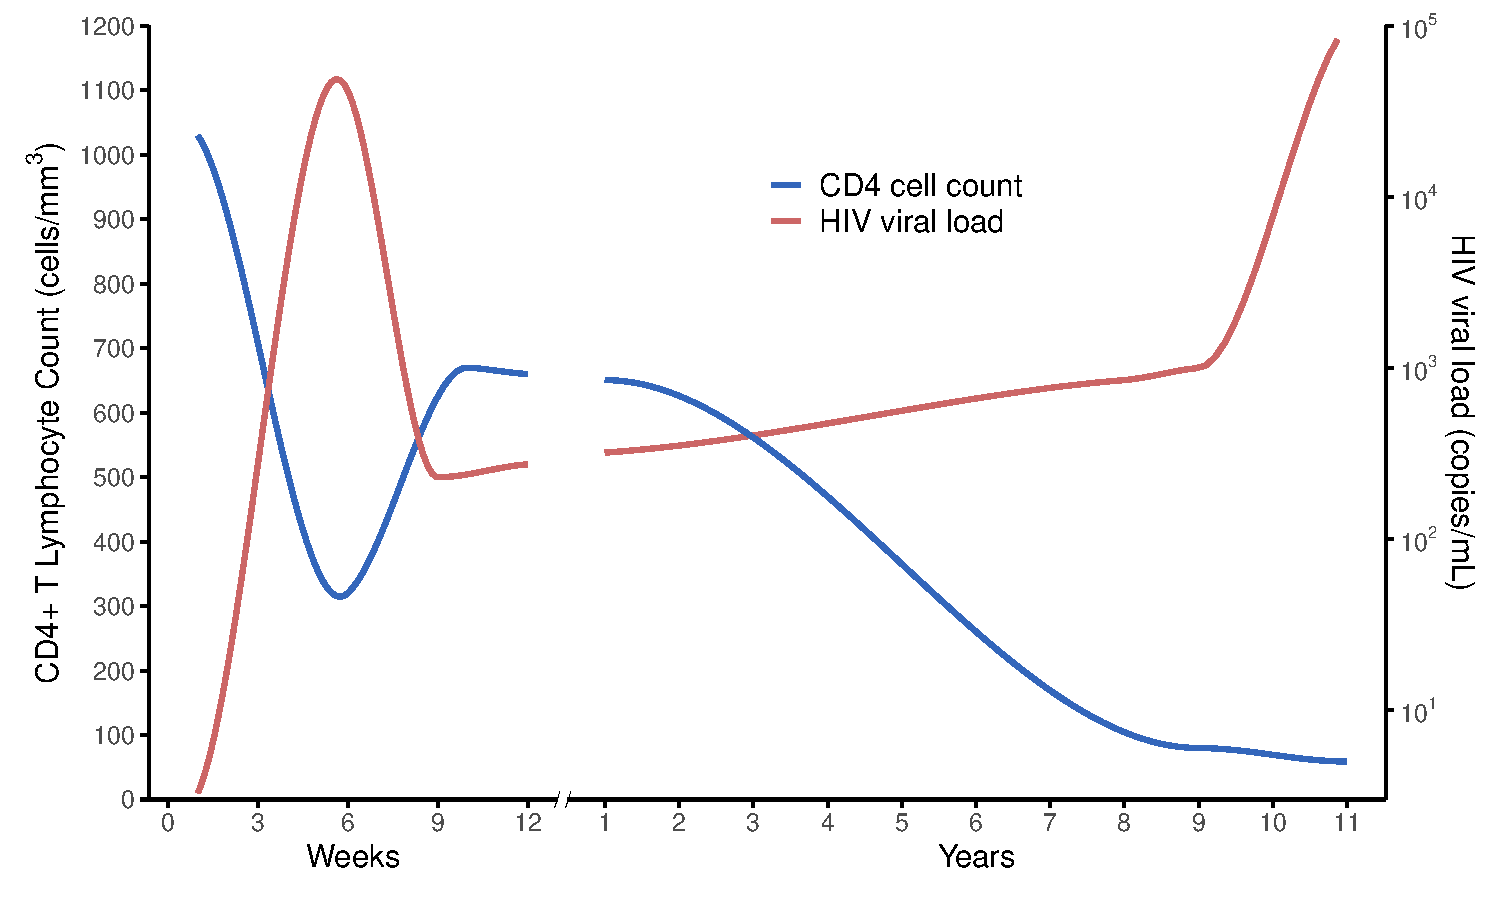
\includegraphics[width=\textwidth]{cd4_trajectory.pdf}
  \caption[CD4 cell count trajectory following HIV infection]{CD4 cell count (cells/mm\textsuperscript{3}) and HIV viral load (copies/mL) trajectories following HIV infection. Figure adapted from~\cite{Maartens2014-xd}.}\label{fig:cd4dip}
\end{figure}

Globally, in recognition of the importance of the CD4 marker in determining immune function, most healthcare settings test an individual's CD4 at the point of HIV diagnosis, and at subsequent healthcare visits, with current UK standards of care guidelines recommending annual CD4 measurements as part of routine HIV outpatient follow-up~\parencite{British_HIV_Association2018-ps}. Prior to 2015, a low CD4 count (<350 cells/mm\textsuperscript{3}) was the primary indication for starting ART in the UK\@. In recognition of high adherence to ART, low side-effects of current regimes, and evidence from randomised trials, the CD4-based treatment criteria has since been removed from most European treatment guidelines, meaning that treatment now often starts immediately upon diagnosis~\parencite{Churchill2016-ol, European_AIDS_Clinical_Society2023-rg, INSIGHT_START_Study_Group2015-af}.

Despite changes to treatment guidelines, CD4 remains widely accepted as an important public health measure, with the European Late Presenter Consensus working group definition of `late HIV diagnosis' being a CD4 count <350 cells/mm\textsuperscript{3}, or an AIDS-defining illness at presentation~\parencite{Antinori2011-hg}, a definition adopted by the WHO and European Centre for Disease Prevention and Control (ECDC)\nomenclature[z]{ECDC}{European Centre for Disease Prevention and Control}~\parencite{World_Health_Organisation2010-fk, European_Centre_for_Disease_Prevention_and_Control2020-db}. Late diagnosis rates may be used to evaluate the success of HIV testing strategies, since a decrease in the number and proportion of people diagnosed late alongside sustained or increased testing volumes indicates a trend towards earlier diagnosis~\parencite{Delpech2013-ug}. Reducing late diagnosis is now a priority area for the HIV Action Plan for England 2022-to-2025~\parencite{Department-of-Health-and-Social-Care2021-ee}.

At an individual level, the measurement of CD4 cells is subject to wide variation; immune cells are known to follow a circadian rhythm, are not uniformly distributed in the blood, and respond to foreign antigens (introduced by diet, pathogens in the air, etc.) and stress~\parencite{Keshani2023-ax, Moncivaiz2013-vz}. However, when averaged at a population level with appropriate grouping intervals, progression between subsequent levels of CD4 (post-seroconversion) can be reliably estimated from studies of HIV seroconverters with known dates of HIV acquisition~\parencite{CASCADE_Concerted_Action_on_SeroConversion_to_AIDS_and_Death_in_Europe_Collaboration2000-wd}.

\subsubsection{HIV avidity assays}

As the immune response to HIV develops following infection, the body develops more effective antibodies which bind more tightly. The binding strength, or antibody `avidity', can be measured using avidity assays, and the avidity score used to measure disease progression and distinguish `recent' from `non-recent' HIV acquisition~\parencite{Murphy2008-zu,SEDIA_Biosciences_Corporation2021-hb}. HIV avidity assays are calibrated against a pool of samples with assumed known infection dates to find an appropriate cut-off --- an avidity score below which recent HIV acquisition is likely. Samples with avidity scores falling below this cut-off are then used to estimate a mean duration of recent infection (MDRI)\nomenclature[z]{MDRI}{Mean duration of recent infection} for the specific assay. The MDRI is the average time spent recently infected within a time $T$ post-infection, expressed as:
%
\[
  \Omega_T = \int_0^T{P_R(t) \dif t}
\]

where $P_R(t)$ is the probability of being alive and `recently' infected at time $t$ after infection~\parencite{Kassanjee2012-uj}.

Avidity assays have been shown to be sensitive to severe immunosuppression from advanced disease, use of ART, elite controllers with naturally highly suppressed viral load, co-infections, HIV subtype, and pregnancy, with a false recency rate (FRR)\nomenclature[z]{FRR}{False recency rate} of up to 10\%~\parencite{Suligoi2011-xs}. This misclassification can be minimised if results are considered as part of an algorithm which utilises clinical markers for established infection and treatment status~\parencite{Aghaizu2014-hl}. In England, Wales, and Northern Ireland (EW\&NI)\nomenclature[z]{EW\&NI}{England, Wales, and Northern Ireland}, avidity test results are routinely incorporated with epidemiological data in a recent infection testing algorithm (RITA)\nomenclature[z]{RITA}{Recent infection testing algorithm} to classify new HIV diagnoses as recent or non-recent (see Appendix~\ref{appendix:biomarkers} for further details). The FRR after application of the RITA algorithm has been estimated as 1.9\% (95\% confidence interval 1.0--3.4\%)~\parencite{Aghaizu2018-kk}.

Additional biomarkers collected as part of routine HIV surveillance in the UK include viral load, p24 antigen and HIV testing history, described in Appendix~\ref{appendix:biomarkers}.

\subsection{UK HIV case surveillance}\label{sec:hiv-surveillance}

Surveillance of HIV in the UK began in 1982, with the first case reports of AIDS to the Communicable Disease Surveillance Centre (CDSC)\nomenclature[z]{CDSC}{Communicable Disease Surveillance Centre}, one of the predecessors of UKHSA\@. Reporting of new HIV diagnoses was introduced after the first test for HIV became available in the UK in 1984~\parencite{British_Broadcasting_Company1984-sk}.

Reports of new HIV diagnoses have been collected ever since, with data currently submitted electronically to UKHSA on an annual basis by laboratories and clinicians from a variety of diagnosis settings across EW\&NI~\parencite{Rice2017-pr}. The covariates collected for new HIV diagnoses include demographic information:\ sex, age, ethnicity, country of birth, probable route of HIV exposure; and diagnosis data:\ setting of diagnosis and first CD4 count and date of CD4 test. All reports of HIV diagnoses are validated against a set of rules, for example:\ no partial dates are accepted and records missing key demographic identifiers are not added to the database. Data cleaning, validation, and de-duplication takes place yearly and records are retained in an annual archive~\parencite{Public_Health_England2013-ma}.

\subsubsection{Biomarker data}

National surveillance of HIV in EW\&NI includes enhanced reporting of biomarker data, with an established record linkage algorithm used to match these biomarker data to HIV diagnosis records for the annual data archive~\parencite{Rice2017-pr, Winter2016-ue}.

The CD4 surveillance scheme, established in 1995, collects longitudinal CD4 count data from 60 laboratories to allow for monitoring of late HIV diagnosis, immunosuppression, and to evaluate the effects of ART~\parencite{Public_Health_England2013-zl}. Samples for HIV avidity testing, alongside pseudonymised demographic information, have been collected centrally by UKHSA since 2011. Avidity testing is used for public health monitoring of the proportion of HIV infections acquired recently, and at the individual level to inform the management of HIV conditions~\parencite{Aghaizu2014-hl}.

Avidity assays have been used for around half of all new HIV diagnoses in EW\&NI over this period, with two avidity assays used:\ the HIV 1/2gO AxSYM assay was used for tests carried out between 2011--2013~\parencite{Suligoi2002-di}, and the Sedia Limiting Antigen Avidity Enzyme Immunoassay (LAg-Avidity EIA)\nomenclature[z]{LAg-Avidity EIA}{Limiting Antigen Avidity Enzyme Immunoassay} used between 2013--2022~\parencite{Sedia_Biosciences_Corporation2013-ff}. The MDRI on a sample taken within 120 days of HIV diagnosis and prior to ART initiation is around 6 months for both assays\footnote{An AxSYM avidity index score <80.0\% has an estimated MDRI of 202 days (95\% credible interval (CrI)\nomenclature[z]{CrI}{Credible interval} 174--245 days)~\parencite{Sweeting2010-hm}. A Sedia LAg with normalised optical density score <1.5 has an estimated MDRI of 188 days (95\% confidence interval 165--211)~\parencite{Kassanjee2014-gc}.}.

\subsection{HIV epidemic models}

\subsubsection{Back-calculation}

As with most infectious diseases, individuals presenting with HIV-related symptoms will typically be tested and receive a diagnosis. Provided an estimate of the incubation period (i.e.\ the time from exposure to symptoms) is available, this can be combined with observed data on diagnoses to `back-calculate' the incidence of infection. The general idea of back-calculation is that the time of symptom onset for an infected person is equal to the sum of the time of exposure and the incubation period~\parencite{Egan2015-oi}. In continuous time this can be expressed by the following convolution:
%
\[
  d(t) = \int_{t_0}^t{h(s)f(t-s) \dif s}
\]

where $d(t)$ is the rate of diagnosis at time $t$, $t_0$ is the starting time of the epidemic, $h(s)$ is the rate of new infections at time $s$, and $f(t-s)$ is the incubation distribution~\parencite{Brookmeyer1994-nr}.

The occurrence of infections over time is typically modelled as a non-homogeneous Poisson process with the number of new infections in a particular time interval being i.i.d. Poisson random variables with mean $h(s)$~\parencite{Becker1991-wj, Rosenberg1991-by}. As linear combinations of Poisson random variables are themselves Poisson-distributed, so the number of new diagnoses is Poisson distributed with mean $d(t)$~\parencite{Chiang1980-yt}.

The back-calculation method was first developed to estimate HIV prevalence from AIDS cases, with the incubation distribution representing the time from HIV exposure to onset of AIDS~\parencite{Brookmeyer1988-va}. With the introduction of HIV testing, individuals could be diagnosed before AIDS symptoms became apparent and the back-calculation model was therefore extended to consider pre-AIDS diagnoses. This extension introduced a time-dependent incubation distribution, $f(t-s \mid s)$, to capture changes in testing~\parencite{Aalen1997-jh}. Further extensions of the model have incorporated HIV progression estimates from CD4 count data to better characterise the time between infection and diagnosis and to estimate trends in the probability of HIV diagnosis by disease stage~\parencite{Birrell2012-hw, Sweeting2005-sj, van-Sighem2015-zo}.

In 2019,~\cite{Brizzi2019-yj} extended the model to include age-specific HIV incidence, allowing for the estimation of age groups at higher risk of HIV infection. Estimates from this model have recently provided evidence of a fall in HIV transmission among GBM, with an estimated 80\% reduction in the incidence of new HIV infection between 2011 and 2019, concentrated among younger GBM~\parencite{Brizzi2021-zl}.

\subsubsection{Approaches to HIV incidence estimation}

Back-calculation models have been used to estimate HIV incidence from diagnosis data in England, Italy, and Australia~\parencite{Bellocco2000-wk, Cui2000-ma, Aalen1997-jh}, with a CD4-staged back-calculation model recently adapted for use in European Union (EU)\nomenclature[z]{EU}{European Union} member states~\parencite{Regine2018-rm, van-Sighem2015-zo, van-Sighem2017-ye}. Aside from back-calculation, several other approaches to HIV incidence estimation exist.

Multi-parameter evidence synthesis (MPES)\nomenclature[z]{MPES}{Multi-parameter evidence synthesis} is a Bayesian approach which combines HIV and sexually transmitted infection (STI)\nomenclature[z]{STI}{Sexually transmitted infection} data sources to estimate serial HIV prevalence rates in key populations~\parencite{Goubar2008-dd, Presanis2021-pv}. Whilst typically used to infer undiagnosed HIV prevalence in the UK, MPES can be applied to estimate HIV incidence, parameterised in terms of prevalence and contact rates~\parencite{Presanis2011-uy}.

Methods to derive HIV incidence from cross-sectional serological assays which detect recent infection, e.g.\ the p24 antigen or BED capture enzyme immunoassay, were first proposed in 1995~\parencite{Brookmeyer1995-ws}, and have since been implemented in a number of countries, including Brazil, the United States, and across sub-Saharan Africa~\parencite{Hall2008-ze, Le-Vu2008-up, Karita2007-sd}. Given concerns about the accuracy of these tests, approaches which consider multiple biomarkers have been developed with the aim of minimising misclassification of recent infection. These methods incorporate CD4 counts, HIV viral loads, and avidity assays alongside the p24 antigen assay~\parencite{Brookmeyer2013-mf, Sun2020-lt}.

An individual-based stochastic simulation model, calibrated to multiple sources of data, has been used to estimate HIV incidence in the UK~\parencite{Phillips2015-jc}. Most recently this model was applied to explore the contribution of earlier treatment initiation and expanded testing in reducing HIV incidence~\parencite{Cambiano2023-lj}.

Finally, the Joint United Nations Programme on HIV/AIDS (UNAIDS) Spectrum model is used nationally and internationally to provide annual estimates of HIV mortality and incidence, particularly in countries with high prevalence of paediatric HIV\@. Spectrum utilises HIV diagnoses in antenatal settings, testing policy and ART coverage information from surveillance and survey data in a joint statistical and mathematical model~\parencite{Stover2019-zm}.

\section{CD4-staged back-calculation model}\label{sec:cd4-backcalc}

The CD4-staged back-calculation model is a Bayesian, discrete-time, multi-state model~\parencite{Birrell2012-hw}. A diagram of states and transitions for the model is shown in Figure~\ref{fig:originalmodel}.
\newline

\begin{figure}[htbp!]
  \centering
  \footnotesize
  \begin{tikzpicture}
    % Nodes
    \node[] (n0) at (0,0) {};
    \node[rstate, align=center] (n1) [right = of n0] {CD4$\geq$500\\($e_{1,j}$)};
    \node[rstate, align=center] (n2) [right = of n1] {CD4 350--499\\($e_{2,j}$)};
    \node[rstate, align=center] (n3) [right = of n2] {CD4 200--349\\($e_{3,j}$)};
    \node[rstate, align=center] (n4) [right = of n3] {CD4<200\\($e_{4,j}$)};
    \node[state, align=center] (n5) [right = of n4] {AIDS\\($\mu_{5,j}$)};
    \node[state, align=center] (n6) [below = of n1] {CD4$\geq$500\\($\mu_{1,j}$)};
    \node[state, align=center] (n7) [below = of n2] {CD4 350--499\\($\mu_{2,j}$)};
    \node[state, align=center] (n8) [below = of n3] {CD4 200--349\\($\mu_{3,j}$)};
    \node[state, align=center] (n9) [below = of n4] {CD4<200\\($\mu_{4,j}$)};
    % Edges
    \path (n0) edge node[above] {$h_j$} (n1);
    \path (n1) edge node[above] {$q_1$} (n2);
    \path (n2) edge node[above] {$q_2$} (n3);
    \path (n3) edge node[above] {$q_3$} (n4);
    \path (n4) edge node[above] {$q_4$} (n5);
    \path (n1) edge[dashed] node[left] {$d_{1,j}$} (n6);
    \path (n2) edge[dashed] node[left] {$d_{2,j}$} (n7);
    \path (n3) edge[dashed] node[left] {$d_{3,j}$} (n8);
    \path (n4) edge[dashed] node[left] {$d_{4,j}$} (n9);
  \end{tikzpicture}
  \caption[CD4-staged back-calculation model]{CD4-staged back-calculation model. Rounded boxes indicate latent (or undiagnosed) states, square boxes indicate diagnosed states. Solid lines indicate HIV progression. Dashed lines indicate transition from latent to diagnosed state.}\label{fig:originalmodel}
\end{figure}

In this model HIV infections are assumed to occur according to a non-homogeneous Poisson process with rate $\lambda(t)$. The expected number of infections in the time interval $(t_{j-1},t_j]$ is given by:
%
\[
  h_j = h(t_j) = \int_{t_{j-1}}^{t_j}\lambda(t) \dif t
\]

Following infection, state transitions proceed on a quarterly (i.e.\ 3-monthly) time interval, with individuals assumed to steadily progress through four latent (or undiagnosed) states $e_{i,j}$ (where $i$ indexes the state), defined by progressively lower CD4 counts. At each CD4 stage, $i$, individuals are subject to differing, time-dependent, diagnosis probabilities $d_{i,j}$. In the absence of a diagnosis individuals will progress to an eventual AIDS state~\parencite{Birrell2012-hw}.

The transition matrix:
%
\[
  \mathbf{Q}_j = \begin{bmatrix}
    (1-d_{1,j})(1-q_1) & (1-d_{1,j})q_1     & 0                  & 0                  \\
    0                  & (1-d_{2,j})(1-q_2) & (1-d_{2,j})q_2     & 0                  \\
    0                  & 0                  & (1-d_{3,j})(1-q_3) & (1-d_{3,j})q_3     \\
    0                  & 0                  & 0                  & (1-d_{4,j})(1-q_4)
  \end{bmatrix}
\]

describes the probability of progression between the latent states of the model during the time interval $(t_{j-1},t_j]$. Here $q_i$ are fixed constant progression probabilities --- from one latent state to the next, estimated from studies of HIV seroconverters~\parencite{CASCADE_Concerted_Action_on_SeroConversion_to_AIDS_and_Death_in_Europe_Collaboration2000-wd}; and $d_{i,j}$ are diagnosis probabilities --- from a latent state to a diagnosed state. A second transition matrix:
%
\[
  \mathbf{D}_j = \begin{bmatrix}
    d_{1,j} & 0       & 0       & 0       & 0              \\
    0       & d_{2,j} & 0       & 0       & 0              \\
    0       & 0       & d_{3,j} & 0       & 0              \\
    0       & 0       & 0       & d_{4,j} & (1-d_{4,j})q_4
  \end{bmatrix}
\]

describes the probability of moving between a latent state and a diagnosed state during time interval $(t_{j-1},t_j]$. The final column of $\mathbf{D}_j$ describes the probability of being diagnosed with AIDS;\ the implicit assumption is that all people who progress to AIDS will be diagnosed.

Denote as $\bm{e}_j = (e_{1,j},\dots,e_{4,j})$ the expected number of individuals in $(t_{j-1},t_j]$ in each of the latent states, and as $\bm{\mu}_j = (\mu_{1,j},\dots,\mu_{5,j})$ the expected number of new diagnoses in $(t_{j-1},t_j]$ in each of the diagnosed states. The model dynamics may be expressed as a set of recursive equations which include the transition matrices defined above:
%
\begin{align*}
  \bm{e}_j   & = \mathbf{Q}_j^\mathsf{T} \bm{e}_{j-1} + {[h_j, 0, \ldots,0]}^\mathsf{T} \\
  \bm{\mu}_j & = \mathbf{D}_j^\mathsf{T} \bm{e}_{j-1}
\end{align*}

The expected number of HIV and AIDS diagnoses in $(t_{j-1},t_j]$ are denoted, respectively, as:
%
\[
  \mu_j^\text{H} = \sum_{i=1}^4{\mu_{i,j}} \: \text{ and } \:
  \mu_j^\text{A} = \mu_{5,j}
\]

\subsection{Likelihood}

The number of new infections in each time interval $(t_{j-1},t_j]$ form a set of independent Poisson random variables with mean $h_j$, for $j = 1,\ldots,N$. At any time interval during the surveillance period individuals with HIV will be in one of three states:
%
\begin{enumerate}
  \item diagnosed with HIV;
  \item diagnosed with AIDS;
  \item undiagnosed.
\end{enumerate}

By the properties of the non-homogeneous Poisson process, the likelihood contributions of the HIV and AIDS diagnoses are given by independent Poisson random variables $Y^\text{H}_j$ and $Y^\text{A}_j$ with expectations $\mu_j^H$ and $\mu_j^A$, respectively:
%
\begin{align*}
  Y^\text{H}_j & \sim \text{Poisson}(\mu_j^\text{H}) \\
  Y^\text{A}_j & \sim \text{Poisson}(\mu_j^\text{A})
\end{align*}

Denote the observed data on HIV and AIDS diagnoses in time interval $(t_{j-1},t_j]$ as $y_j^\text{H}$ and $y_j^\text{A}$, with $\bm{y}^\text{H} = (y_1^\text{H}, \ldots, y_N^\text{H})$ and $\bm{y}^\text{A} = (y_1^\text{A}, \ldots, y_N^\text{A})$. These are realisations of Poisson random variables, so the likelihood contribution from these data is:
%
\[
  L_1(\bm{y}^\text{H}, \bm{y}^\text{A};\bm{h},\bm{d}) \propto \prod_{j=1}^T {(\mu_j^\text{A})}^{y^\text{A}_j}\exp(-\mu_j^\text{A})\times{(\mu_j^\text{H})}^{y^\text{H}_j}\exp(-\mu_j^\text{H})
\]

Then, for each of the four CD4 states, let $Y^\text{C}_{i,j}$ be the random variable for the number of HIV diagnoses in state $i$ in time interval $(t_{j-1},t_j]$. These diagnoses are multinomially distributed, with CD4 counts assumed to be missing at random, so:
%
\[
  Y^\text{C}_{i,j} \sim \text{Multinomial}(n_j,\bm{c}_j)
\]

where $\bm{c_j}$ is the parameter set of expected probabilities in each CD4 diagnosis state:
%
\[
  \bm{c}_j = \left(\frac{\mu_{1,j}}{\mu_j^\text{H}},\frac{\mu_{2,j}}{\mu_j^\text{H}},\frac{\mu_{3,j}}{\mu_j^\text{H}},\frac{\mu_{4,j}}{\mu_j^\text{H}}\right)
\]

$n_j$ is the observed total number of HIV diagnoses in $(t_{j-1},t_j]$ with CD4 count data available:
%
\[
  n_j = \sum_{i=1}^4{y^\text{C}_{i,j}} \subseteq y^\text{H}_j
\]

and $y_{i,j}^\text{C}$ are the observed CD4 data in each CD4 diagnosis state $i$, and time interval $(t_{j-1},t_j]$, with $\bm{y}^\text{C} = \{y_{i,j}^\text{C}:\; i = 1,\ldots,4, j = 1,\ldots,N\}$.

The likelihood contribution from the observed CD4 data is therefore:
%
\[
  L_2(\bm{y^{\text{C}}} \mid \bm{y^\text{H}};\bm{h},\bm{d})\propto \prod_{j=1}^T \prod_{i=1}^4 {(c_{i,j})}^{y^{\text{C}}_{i,j}}
\]

and the full likelihood for this model is the product of the two likelihood terms:
%
\[
  L(\bm{y^\text{H}}, \bm{y^\text{A}},\bm{y^{\text{C}}};\bm{h},\bm{d}) = L_1(\bm{y}^\text{H}, \bm{y}^\text{A};\bm{h},\bm{d}) \times L_2(\bm{y^{\text{C}}} \mid \bm{y^\text{H}};\bm{h},\bm{d})
\]

\subsection{Smoothing incidence and diagnosis trends}

To address identifiability issues, the time-varying infection ($\bm{h}$) and diagnosis ($\bm{d}$) rates are specified according to random-walks on the log-scale. Prior distributions are chosen as an uninformative $\text{Gamma}(1,32)$ for the variance of the random walks, a Normal distribution focused at $\log(2)$ for the starting point of the incidence random walk, and according to results of an earlier study for the mean of the diagnosis random walk at 1985, with a ramp up to this level for previous years~\parencite{Aalen1997-jh, Birrell2013-va}. This specification serves to smooth these processes over time, ensuring that sudden jumps do not occur between time intervals~\parencite{Birrell2012-hw}. Alternate parametric smoothing methods for the incidence and diagnosis rates may be specified, e.g.\ Gaussian processes or various spline models~\parencite{Brizzi2017-fv}.

In the Bayesian framework the priors are updated by the likelihood to obtain the posterior. As the posterior in this case is intractable, samples are obtained via a suitable MCMC algorithm (e.g.\ as implemented in the JAGS or STAN software).

\subsection{Latent states}

Let $Y^\text{E}_{i,j}$ be the random variable for the number of individuals in each of the four latent states after time interval $(t_{j-1},t_j]$, with expectation $e_{i,j}$. To make statements about these latent states whilst accounting for the full uncertainty about the number of individuals in each state, the \textit{posterior predictive} distribution for the unobserved $\bm{y}^\text{E} = \{y_{i,j}^\text{E}:\; i = 1,\ldots,4, j = 1,\ldots,N\}$ is needed. This posterior predictive distribution is calculated by marginalising over the posterior distribution of the model parameters, $\theta=(\bm{h},\bm{d})$, given the data:
%
\begin{align*}
  \pi(\bm{y}^\text{E} \mid \bm{y}^\text{H},\bm{y}^\text{A},\bm{y}^\text{C}) = \int_\Theta p(\bm{y}^\text{E} \mid \bm{y}^\text{H},\bm{y}^\text{A},\bm{y}^\text{C},\theta) \pi(\theta \mid  \bm{y}^\text{H},\bm{y}^\text{A},\bm{y}^\text{C}) \dif\theta
\end{align*}

where $\pi(.)$ represents a posterior probability distribution. The distribution $p(\bm{y}^\text{E} \mid \bm{y}^\text{H},\bm{y}^\text{A},\bm{y}^\text{C},\theta)$ is a non-standard distribution, and computationally expensive to simulate from. Instead, `post-hoc' methods may be used to derive quantities of interest which involve the posterior predictive distribution for $\bm{y}^\text{E}$. For instance, by expressing undiagnosed HIV prevalence as the total number of infections minus the number of HIV and AIDS diagnoses~\parencite{Birrell2012-hw}.

\subsection{Limitations}

Despite the successful application of the existing CD4 back-calculation model to reveal changes in incidence which precede an observed fall in diagnoses~\parencite{Brizzi2021-zl}, the approach has certain limitations which affect both the precision and relevance of estimates for continued HIV incidence estimation.

\subsubsection{Misclassification of longstanding infection}

The success of combination HIV prevention initiatives during the past decade have led to a higher frequency of testing among those most at risk of infection~\parencite{Brown2017-yu}. Over the same period, more sensitive `fourth-generation' HIV tests, capable of detecting the virus earlier in infection, were recommended for routine use in the UK~\parencite{National_Institute_for_Health_and_Care_Excellence2016-us}. As a result, the probability of HIV diagnosis occurring during the acute phase of infection (when CD4 counts are prone to dip) is likely to have increased substantially. In a recent Belgian study, for example, a third of people diagnosed with recently-acquired infection had a CD4 count below 350 cells/mm\textsuperscript{3}~\parencite{Sasse2016-gh}. Whilst a trend towards earlier diagnosis is undoubtedly a positive for HIV prevention, and beneficial at an individual-level, the use of CD4 counts at diagnosis to measure progression towards AIDS may be increasingly subject to error.

The CD4 back-calculation model does not account for a transient dip in CD4 cell counts during acute infection. And while similar CD4-staged HIV estimation approaches have included a `primary infection' stage, individuals are not assumed to be diagnosed during this stage~\parencite{van-Sighem2015-zo}. The issue of CD4 counts dipping early in infection is also a challenge for determining population-level late HIV diagnosis rates, as highlighted by UK and other European reports~\parencite{HIV_Commission2020-yy, Sasse2016-gh, Brannstrom2016-nx}.

\subsubsection{Uncertainty in recent incidence estimates}

A second limitation of the back-calculation model stems from the high variability of CD4 cell counts and, as a result, the necessary imprecision of CD4 strata used in the model. In particular, there is a wide time interval following HIV seroconversion during which CD4 cell counts may remain above 500 cells/mm\textsuperscript{3} (around 3 years)~\parencite{Maartens2014-xd}. This is particularly evident in recent years which, crucially, are those used to assess current progress towards elimination of HIV transmission.

\begin{figure}[htbp!]
  \centering
  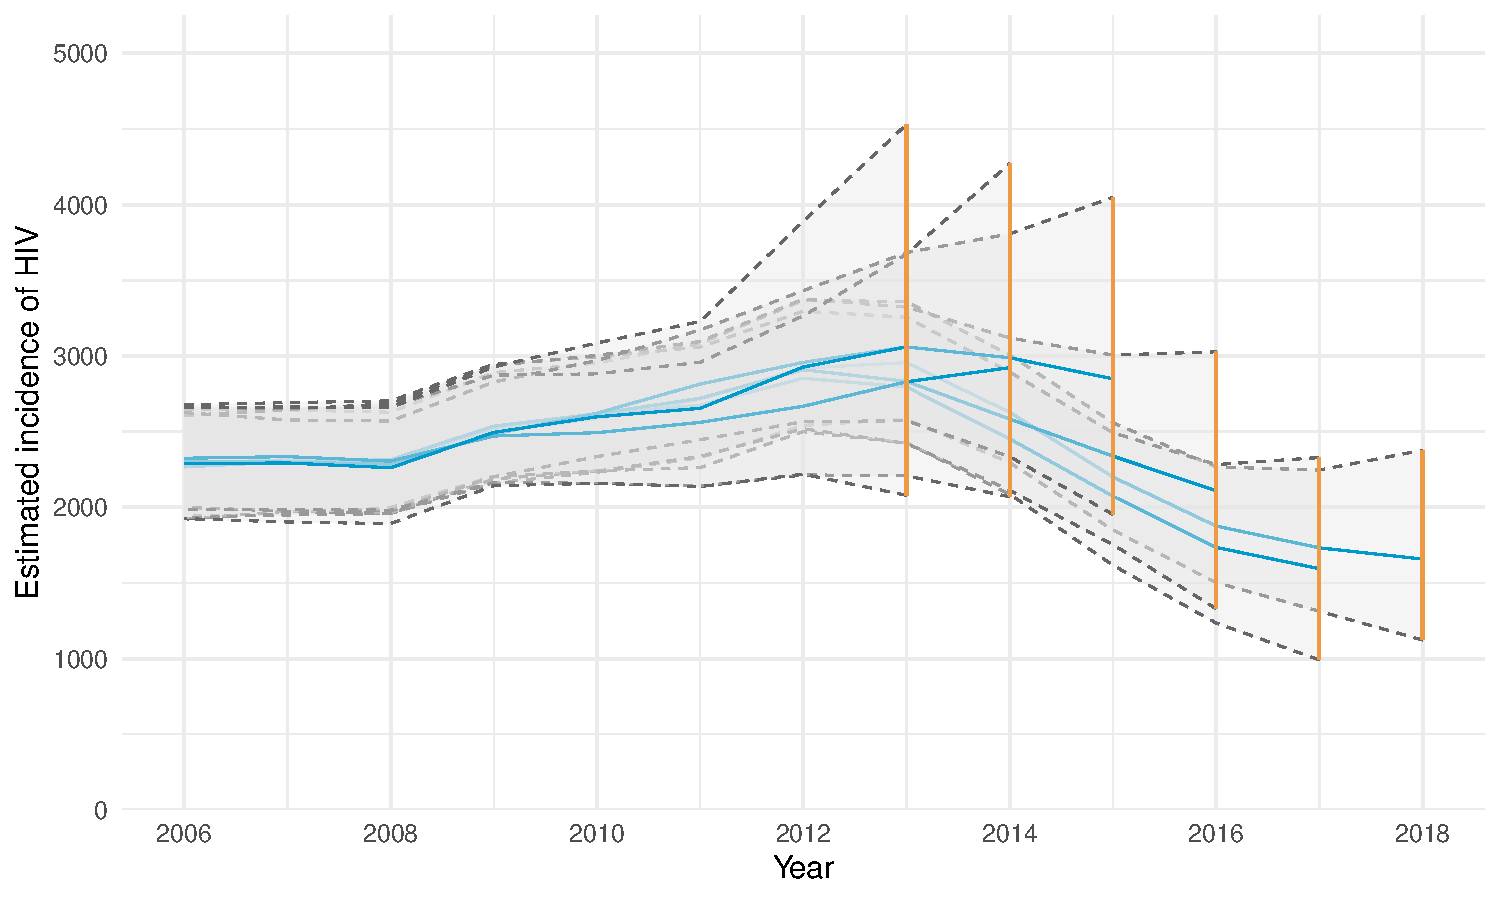
\includegraphics[width=\textwidth]{incidence_overlay_2014_2018.pdf}
  \caption[Successive annual estimates of HIV incidence (posterior median and 95\% CrI) estimated by CD4 back-calculation]{Successive annual estimates of HIV incidence (posterior median and 95\% CrI) estimated by CD4 back-calculation. The vertical line indicates the range of the credible interval for the the most recent year of available diagnosis data.}\label{fig:wideintervals}
\end{figure}

As shown in Figure~\ref{fig:wideintervals}, for successive annual estimates of HIV incidence estimates the credible intervals are widest for the most recent 2--3 years, narrowing as subsequent diagnosis information becomes available. Being able to better discern the recency of a newly diagnosed infection may help to improve the precision of incidence estimation.
\newline

Incorporating other biomarkers of recent infection (such as those described in Section~\ref{sec:biomarkers}) could help to address both limitations:\ complementing the CD4 cell count by detecting acute and/or early HIV infection, and improving the precision and identifiability of the model for the most recent years.

The extent of CD4 misclassification has not been previously investigated for UK data. In the next section I investigate the availability and representativeness of the available biomarker data, then use these markers to quantify to what extent an HIV diagnosis occurring during the acute or seroconversion phase may be misclassified as a `late diagnosis' (due to being diagnosed with a CD4 count <350 cells/mm\textsuperscript{3}).

\section{Analysis of biomarker data}

An initial investigation of the availability and representativeness of HIV viral loads, HIV avidity assays, and HIV testing history for 10 years of diagnosis data among GBM in EW\&NI was undertaken. The key findings are summarised below, with full results included in Appendix~\ref{appendix:biomarker-availability}.

\subsection{Key findings}

Based on HIV avidity assay results and HIV testing history, an increasing proportion of newly diagnosed GBM with low CD4 counts (<350 cells/mm\textsuperscript{3}) were found to have evidence of recent HIV acquisition; around a quarter in 2019 compared to <10\% in 2011. This finding was corroborated by viral load information --- an increasing proportion of those diagnosed with recent infection had elevated baseline viral loads (>100,000 copies/mL), suggestive of diagnosis during acute infection, at a time of peak viremia.

The results of the biomarker data were somewhat age-dependent, with the avidity assay analyses suggesting that younger GBM were more likely than older GBM to be diagnosed promptly. Availability of previous negative test data was similarly age-dependent, with a higher proportion of GBM aged <50 having previous negative tests within 6 months of their HIV diagnosis, compared to older GBM\@. This reflects the concentration of HIV-prevention campaigns, and high testing volumes at SHS (and therefore greater likelihood of being diagnosed during seroconversion) for younger age groups~\parencite{Whitlock2020-aa}.

Despite excluding individuals known to have initiated treatment, an increasing proportion of newly diagnosed GBM had a baseline viral load <50 copies/mL, highly suggestive of viral suppression due to ART\@. Whilst this may be due in part to missing information on treatment start date, widespread use of PrEP among GBM may result in viral load suppression at diagnosis for the small number of breakthrough cases~\parencite{Ambrosioni2021-es}. Since ART, post-exposure prophylaxis (PEP)\nomenclature[z]{PEP}{Post-exposure prophylaxis}, and PrEP all affect the measurement of avidity, the application of the RITA algorithm (which accounts for both viral load and treatment start information) will be necessary to maintain a low false recency rate (FRR).

\subsection{Revised late HIV diagnosis definition}\label{sec:ld-reassessment}

The public health definition of late HIV diagnosis is a CD4 cell count <350 cells/mm\textsuperscript{3}.  The population-level late diagnosis rate is an important public health measure used to target HIV-prevention initiatives, such as testing campaigns, ART initiation, and PrEP~\parencite{Brown2017-yu, Churchill2016-ol, NHS_England2019-gt}, and a key indicator of the English Public Health Outcomes Framework~\parencite{Office_for_Health_Improvement2023-xd}.

Based on the analysis of HIV biomarker data in this section, the CD4<350 cells/mm\textsuperscript{3} definition will increasingly overestimate rates of late HIV presentation in EW\&NI\@. To address this overestimation I developed a reclassification method in collaboration with colleagues at UKHSA\@. This method incorporates routine tests for recent infection and evidence of a recent negative HIV test into the measurement of population-level late diagnosis rates, with the revised definition of late HIV diagnosis below~\parencite{Kirwan2022-za}.

\begin{framed}
  \begin{quote}
    \textbf{Revised definition of late HIV diagnosis}

    Among adults (aged $\geq$15 years) with a baseline CD4 count (within  14 to 91 days), those with a CD4 count <350 cells/mm\textsuperscript{3} and neither:
    \begin{itemize}
      \item[(a)] a  recent  infection  testing  algorithm (RITA) result indicating recent HIV acquisition nor
      \item[(b)] a negative HIV test result within the preceding 24 months.
    \end{itemize}
  \end{quote}
\end{framed}

The impact of the revised late HIV diagnosis definition on late diagnosis rates in EW\&NI is described in Appendix~\ref{appendix:late-diag}. The updated definition is now routinely used for public health monitoring at English local authority-level~\parencite{Office_for_Health_Improvement2023-xd}, at national level~\parencite{Martin2023-um}, and has informed an updated European consensus definition of late HIV diagnosis~\parencite{Croxford2022-cv}.

These findings motivate the next section of this chapter, where avidity test information will be introduced as an additional biomarker for the CD4 back-calculation, with the aim of improving model performance and addressing the misclassification of recent infection.

\section{Dual biomarker back-calculation model}

In this section, I propose an updated `dual biomarker' back-calculation model for HIV incidence estimation, incorporating both CD4 cell count and HIV avidity test information. The model is described in detail below, followed by a simulation study to explore the performance of the dual biomarker model compared to the original CD4 back-calculation model. The updated version of the back-calculation model is then applied to HIV surveillance data for England.

Of the available biomarkers, the avidity assay biomarker had the least bias in data availability, the RITA algorithm helped to mitigate false recency error, and data were derived from independently-reported laboratory samples. The HIV testing history data, meanwhile, had greater age-dependency, with an unknown degree of error in recall and reporting, and these data were subject to external factors such as HIV testing campaigns and expanded point-of-care testing.

\subsection{Model description}\label{sec:dual-biomarker-model}

\subsubsection{Addition of recently acquired HIV states}

The addition of a recent state to the CD4 back-calculation model should, conceptually, allow for progression through an additional `recently acquired' latent state, and corresponding diagnosed state, as shown in Figure~\ref{fig:naiverita}, where the (time-varying) probability of diagnosis is $d_{1,j}$.

\begin{figure}[htbp!]
  \centering
  \footnotesize
  \begin{tikzpicture}
    \path (0,0.4);
    \path (0,-2.7);
    % Nodes
    \node[] (n0) at (0,0) {};
    \node[rstate, align=center] (a1) [right = of n0] {Recently acquired \\ HIV ($\leq$6 months)};
    \node[state, align=center] (r1) [below = of a1] {Recently acquired \\ HIV ($\leq$6 months)};
    \node[align=center] (a2) [right = 20mm of a1] {Non-recent \\ HIV (>6 months)};

    % Edges
    \path (n0) edge node[above] {$h_j$} (a1);
    \path (a1) edge node['] {} (a2);

    \path (a1) edge[dashed] node[] {$d_{1,j}$} (r1);

  \end{tikzpicture}
  \caption[Recently acquired state for HIV back-calculation model]{Recently acquired state for HIV back-calculation model. Rounded boxes indicate latent states, square boxes indicate diagnosed states. Solid lines indicate HIV progression. Dashed lines indicate transition from latent to diagnosed state.}\label{fig:naiverita}
\end{figure}

The MDRI for a recent avidity assay result has previously been estimated as around 6 months, which covers two discrete time steps in the model~\parencite{Sweeting2010-hm, Kassanjee2014-gc}. For consistency with the CD4 back-calculation and data reporting mechanisms, it is desirable to retain the quarterly timescale. To accomplish this, the recently acquired HIV latent state is divided in two, reflecting 0--3 and 3--6 months post-HIV acquisition, respectively, as shown in Figure~\ref{fig:rita2latentstates}. The same time-varying probability of diagnosis into a single diagnosis state ($d_{1,j}$) is applied for both latent states.

\begin{figure}[htbp!]
  \centering
  \footnotesize
  \begin{tikzpicture}
    \path (0,0.4);
    \path (0,-2.7);
    % Nodes
    \node[] (n0) at (0,0) {};
    \node[rstate, align=center] (a1) [right = of n0] {Within 0-3 months \\ of HIV acquisition};
    \node[state, align=center] (r1) [below right= 10mm and -5mm of a1] {Recently acquired \\ HIV ($\leq$6 months)};
    \node[rstate, align=center] (a2) [above right= 10mm and -5mm of r1] {Within 3-6 months \\ of HIV acquisition};
    \node[align=center] (a3) [right = 20mm of a2] {Non-recent HIV \\ (>6 months)};

    % Edges
    \path (n0) edge node[above] {$h_j$} (a1);
    \path (a1) edge node['] {} (a2);
    \path (a2) edge node['] {} (a3);

    \path (a1) edge[dashed, bend right=20] node['] {$d_{1,j}$} (r1);
    \path (a2) edge[dashed, bend left=20] node[] {$d_{1,j}$} (r1);

  \end{tikzpicture}
  \caption[Recently acquired states for HIV back-calculation model]{Recently acquired states for HIV back-calculation model. Rounded boxes indicate latent states, square boxes indicate diagnosed states. Solid lines indicate HIV progression. Dashed lines indicate transition from latent to diagnosed state.}\label{fig:rita2latentstates}
\end{figure}

Finally, to combine these recently acquired states with the existing CD4-staged states, the CD4 progression probabilities $\bm{q} = (q_1, q_2, q_3, q_4)$ are introduced. In the CD4-staged model progression can occur after 3 months, therefore the latent state `Within 3--6 months of HIV acquisition' is sub-divided, expanding the number of latent states to three, as shown in Figure~\ref{fig:ritamodel}.

\begin{figure}[htbp!]
  \centering
  \footnotesize
  \begin{tikzpicture}
    % Nodes
    \node[] (n0) at (0,0) {};
    \node[rstate, align=center] (a1) [right = of n0] {Acq. 0-3 mo.\\($e_{1,j}$)};
    \node[rstate, align=center] (a2) [below = of a1] {Acq. 3-6 mo.\\($e_{2,j}$)};
    \node[rstate, align=center] (a3) [right = 10mm of a2] {Acq. 3-6 mo.\\($e_{3,j}$)};
    \node[state, align=center] (r1) [right = 50mm of a1] {Recently acquired \\ HIV ($\leq$6 months)\\($\mu_{1,j}$)};

    \node[rstate, align=center] (n1) [below = of a2] {CD4$\geq$500\\($e_{4,j}$)};
    \node[rstate, align=center] (n2) [right = 12mm of n1] {CD4 350-499\\($e_{5,j}$)};
    \node[rstate, align=center] (n3) [right = of n2] {CD4 200-349\\($e_{6,j}$)};
    \node[rstate, align=center] (n4) [right = of n3] {CD4<200\\($e_{7,j}$)};
    \node[state, align=center] (n5) [right = of n4] {AIDS\\($\mu_{6,j}$)};
    \node[state, align=center] (n6) [below = of n1] {Non-recent HIV \\ (>6 months) and \\CD4$\geq$500\\($\mu_{2,j}$)};
    \node[state, align=center] (n7) [below = of n2] {Non-recent HIV \\ (>6 months) and \\CD4 350-499\\($\mu_{3,j}$)};
    \node[state, align=center] (n8) [below = of n3] {Non-recent HIV \\ (>6 months) and \\CD4 200-349\\($\mu_{4,j}$)};
    \node[state, align=center] (n9) [below = of n4] {Non-recent HIV \\ (>6 months) and \\CD4<200\\($\mu_{5,j}$)};
    % Edges
    \path (n0) edge node[above] {$h_j$} (a1);

    \path (a1) edge node['] {$1-q_1$} (a2);
    \path (a1) edge node[pos = 0.75] {$q_1$} (a3);
    \path (a2) edge node['] {$1-q_1$} (n1);
    \path (a2) edge node[] {$q_1$} (n2);
    \path (a3) edge node[] {$1-q_2$} (n2);
    \path (a3) edge node[] {$q_2$} (n3);
    \path (a1) edge[dashed, bend left=20] node[] {$d_{1,j}$} (r1);
    \path (a2) edge[dashed, bend left=20] node[] {$d_{1,j}$} (r1);
    \path (a3) edge[dashed, bend left=20] node[pos = 0.4] {$d_{1,j}$} (r1);

    \path (n1) edge node[] {$q_1$} (n2);
    \path (n2) edge node[] {$q_2$} (n3);
    \path (n3) edge node[] {$q_3$} (n4);
    \path (n4) edge node[] {$q_4$} (n5);
    \path (n1) edge[dashed] node['] {$d_{2,j}$} (n6);
    \path (n2) edge[dashed] node['] {$d_{3,j}$} (n7);
    \path (n3) edge[dashed] node['] {$d_{4,j}$} (n8);
    \path (n4) edge[dashed] node['] {$d_{5,j}$} (n9);
  \end{tikzpicture}
  \caption[Dual biomarker back-calculation model with `recent incidence assay' and `non-recent incidence assay' CD4-staged states]{Dual biomarker back-calculation model with `recent incidence assay' and `non-recent incidence assay' CD4-staged states. Rounded boxes indicate latent states, square boxes indicate diagnosed states. Solid lines indicate HIV progression. Dashed lines indicate transition from latent to diagnosed state. Acq. = Acquired.}\label{fig:ritamodel}
\end{figure}

The sub-division of states ensures that the same CD4 progression probabilities described in Section~\ref{sec:cd4-backcalc} continue to apply for all individuals in the model. Note the change of orientation in Figure~\ref{fig:ritamodel} so that time proceeds in the vertical direction whilst disease progression proceeds in the horizontal direction. Here, again, the probabilities of diagnosis from all of the three latent states are defined to be equal to $d_{1,j}$.

Individuals who are not recently diagnosed progress to one of the previously described CD4 strata with two time periods having elapsed. For an individual who acquired HIV at time $t_j$, the probability of entering CD4 stratum $S$ at time $t_{j+3}$, given they are not recently diagnosed, is:
%
\begin{itemize}
  \item $\Pr(S(t_{j+3}) = \text{CD4 500+} \mid \text{not recently diagnosed}) = (1-q_1)(1-q_1)$
  \item $\Pr(S(t_{j+3}) = \text{CD4 350--499} \mid \text{not recently diagnosed}) = q_1(1-q_1) + q_1(1-q_2)$
  \item $\Pr(S(t_{j+3}) = \text{CD4 200--349} \mid \text{not recently diagnosed}) = q_1 q_2$
  \item $\Pr(S(t_{j+3}) = \text{CD4}<200 \mid \text{not recently diagnosed}) = 0$
\end{itemize}

The transition matrix $\mathbf{Q}_j$ and diagnosis probability matrix $\mathbf{D}_j$ are updated from the CD4 back-calculation as shown below, with diagonal entries $(1,1)$, $(2,2)$, and $(3,3)$ of $\mathbf{Q}_j$ set equal to zero, indicating no retention in these states at the following time step.
%
\[
  \mathbf{Q}_j = \begin{bsmallmatrix}
    0 & (1-d_{1,j})(1-q_1) & (1-d_{1,j})q_1 & 0 & 0 & 0 & 0 \\
    0 & 0 & 0 & (1-d_{1,j})(1-q_1) & (1-d_{1,j})q_1 & 0 & 0 \\
    0 & 0 & 0 & 0 & (1-d_{1,j})(1-q_2) & (1-d_{1,j})q_2 & 0 \\
    0 & 0 & 0 & (1-d_{2,j})(1-q_1) & (1-d_{2,j})q_1 & 0 & 0\\
    0 & 0 & 0 & 0 & (1-d_{3,j})(1-q_2) & (1-d_{3,j})q_2 & 0\\
    0 & 0 & 0 & 0 & 0 & (1-d_{4,j})(1-q_3) & (1-d_{4,j})q_3 \\
    0 & 0 & 0 & 0 & 0 & 0 & (1-d_{5,j})(1-q_4)
  \end{bsmallmatrix}
\]
%
\[
  \mathbf{D}_j = \begin{bsmallmatrix}
    d_{1,j} & 0 & 0 & 0 & 0 & 0 \\
    d_{1,j} & 0 & 0 & 0 & 0 & 0 \\
    d_{1,j} & 0 & 0 & 0 & 0 & 0 \\
    0 & d_{2,j} & 0 & 0 & 0 & 0 \\
    0 & 0 & d_{3,j} & 0 & 0 & 0 \\
    0 & 0 & 0 & d_{4,j} & 0 & 0 \\
    0 & 0 & 0 & 0 & d_{5,j} & (1-d_{5,j})q_4
  \end{bsmallmatrix}
\]

As before:
%
\begin{align*}
  \bm{e}_j   & = \mathbf{Q}_j^\mathsf{T} \bm{e}_{j-1} + {[h_j, 0, \ldots,0]}^\mathsf{T} \\
  \bm{\mu}_j & = \mathbf{D}_j^\mathsf{T} \bm{e}_{j-1}
\end{align*}

and the expected number of HIV diagnoses in the recent and four non-recent states in $(t_{j-1},t_j]$ are expressed, respectively, as:
%
\[
  \mu_j^\text{R} = \mu_{1,j} \: \text{ and } \:
  \mu_j^\text{L} = \sum_{i=2}^5{\mu_{i,j}}
\]

\subsubsection{Likelihood}

Following Section~\ref{sec:cd4-backcalc}, in each time interval $(t_{j-1}, t_j]$, individuals may be in one of four states:
%
\begin{enumerate}
  \item diagnosed with recently acquired HIV, according to RITA ($\leq$6 months);
  \item diagnosed with longstanding HIV, according to RITA (>6 months);
  \item diagnosed with AIDS;
  \item undiagnosed.
\end{enumerate}

Let $Y^\text{R}_j$ and $Y^\text{L}_j$ be binomial and multinomial random variables for the number of recent and longstanding HIV diagnoses, respectively:
%
\begin{align*}
  Y^\text{R}_j     & \sim \text {Binomial}(n_j,r_j)                  \\
  Y^\text{L}_{i,j} & \sim \text {Multinomial}(n_j^\text{L},\bm{l}_j)
\end{align*}

with parameters:
%
\begin{align*}
  n_j          & = y^\text{R}_j + \sum_{i=1}^4{y^\text{L}_{i,j}} \quad \quad \quad
  r_j = \frac{\mu^\text{R}_{j}}{\mu_j^\text{H}}                                    \\
  n^\text{L}_j & = \sum_{i=1}^4{y^\text{L}_{i,j}} \quad \quad \quad \quad \quad
  \bm{l}_j =\left(\frac{\mu_{2,j}}{\mu_j^\text{L}},\frac{\mu_{3,j}}{\mu_j^\text{L}},\frac{\mu_{4,j}}{\mu_j^\text{L}},\frac{\mu_{5,j}}{\mu_j^\text{L}}\right)
\end{align*}

where $y^\text{R}_j$ and $y^\text{L}_{i,j}$ are the observed data on recent diagnoses and longstanding HIV diagnoses in each of the four CD4 states, respectively, in $(t_{j-1},t_j]$.

The previously defined likelihood contribution $L_1$ is retained, the likelihood contribution from the observed CD4 count data ($L_2$) now relates only to those with longstanding HIV, and a third likelihood contribution ($L_3$) is now available from the recent diagnosis data, conditional on $n_j$\@:
%
\begin{align*}
  L_1(\bm{y^\text{H}}, \bm{y^\text{A}};\bm{h},\bm{d})                      & \propto \prod_{j=1}^T {(\mu_j^\text{A})}^{y^\text{A}_j}\exp(-\mu_j^\text{A})\times{(\mu_j^\text{H})}^{y^\text{H}_j}\exp(-\mu_j^\text{H}) \\
  L_2(\bm{y}^\text{L} \mid \bm{y}^\text{R}, \bm{y}^\text{H};\bm{h},\bm{d}) & \propto \prod_{j=1}^T \prod_{i=1}^4 {(l_{i,j})}^{y^{\text{L}}_{i,j}}                                                                     \\
  L_3(\bm{y}^\text{R} \mid \bm{y}^\text{L}, \bm{y}^\text{H};\bm{h},\bm{d}) & \propto \prod_{j=1}^T {(r_j)}^{n_j}
\end{align*}

The full likelihood is the product of all three likelihood terms:
%
\begin{align*}
  L(\bm{y}^\text{H}, \bm{Y}^\text{A},\bm{y}^\text{R}, \bm{Y}^\text{L};\bm{h},\bm{d}) = L_1(\bm{y^\text{H}}, \bm{y^\text{A}};\bm{h},\bm{d}) \times L_2(\bm{y}^\text{L} \mid \bm{y}^\text{R}, \bm{y}^\text{H};\bm{h},\bm{d}) \times L_3(\bm{y}^\text{R} \mid \bm{y}^\text{L}, \bm{y}^\text{H};\bm{h},\bm{d})
\end{align*}

As before, the time-varying $\bm{h}$ and $\bm{d}$ are specified according to parametric smoothing method, with appropriate prior distributions. Similar post-hoc methods to those presented by~\cite{Birrell2012-hw} are used to derive quantities of interest involving the posterior predictive distribution of the latent model states.

\subsubsection{Data representativeness}

By including only diagnoses with both CD4 and RITA information available to inform HIV progression, the assumption being made is that these data are missing at random. The investigation of the HIV avidity data demonstrated considerable regional differences in data availability, e.g.\ particularly low availability in Wales. A certain degree of age-dependency in the availability of avidity information and the classification of recent/non-recent using the RITA algorithm was also seen.

These regional and age dependencies contradict the assumption that data are missing at random. To minimise the effect of regional differences only diagnoses in England will be considered when applying the model to national surveillance data. Meanwhile, the difference in data availability by age is relatively small and unlikely to make a meaningful difference to model results.

\subsection{Simulation study}\label{sec:hiv-simulation}

In this section the results of a simulation study for assessing the performance of the dual biomarker model as compared to the CD4-only model are reported, with a comparison of bias in estimates.

\subsubsection{Aim}

The aim of the simulation study was to assess the performance of the dual biomarker model and CD4-only model in reconstructing HIV incidence and HIV diagnosis probabilities in the context of HIV diagnosis occurring during acute infection.

\subsubsection{Data generating mechanisms}

Data were simulated by propagating infections through the convolution equations and transition matrices for the dual biomarker model, as defined in Section~\ref{sec:dual-biomarker-model}:
%
\begin{align*}
  \bm{e}_j   & = \mathbf{Q}_j^\mathsf{T} \bm{e}_{j-1} + {[h_j, 0, \ldots,0]}^\mathsf{T} \\
  \bm{\mu}_j & = \mathbf{D}_j^\mathsf{T} \bm{e}_{j-1}
\end{align*}

Data were simulated from these equations 100 times, with independent draws according to the following parametric distributions:
%
\begin{itemize}
  \item $h_j \sim \text{Poisson}(\lambda_{j})$, with $\lambda_{j}$ chosen to approximate a previously estimated pattern of HIV incidence in England, as shown in Figure~\ref{fig:lambda_sim} panel A\@;
  \item $d_{i,j} \sim N(\delta_{i,j}, 0.001^2)$, with the $\delta_{i,j}$ chosen to represent a scenario in which probability of diagnosis increases, flattens, then decreases, as shown in Figure~\ref{fig:lambda_sim} panel B\@.
\end{itemize}

\begin{figure}[htbp!]
  \centering
  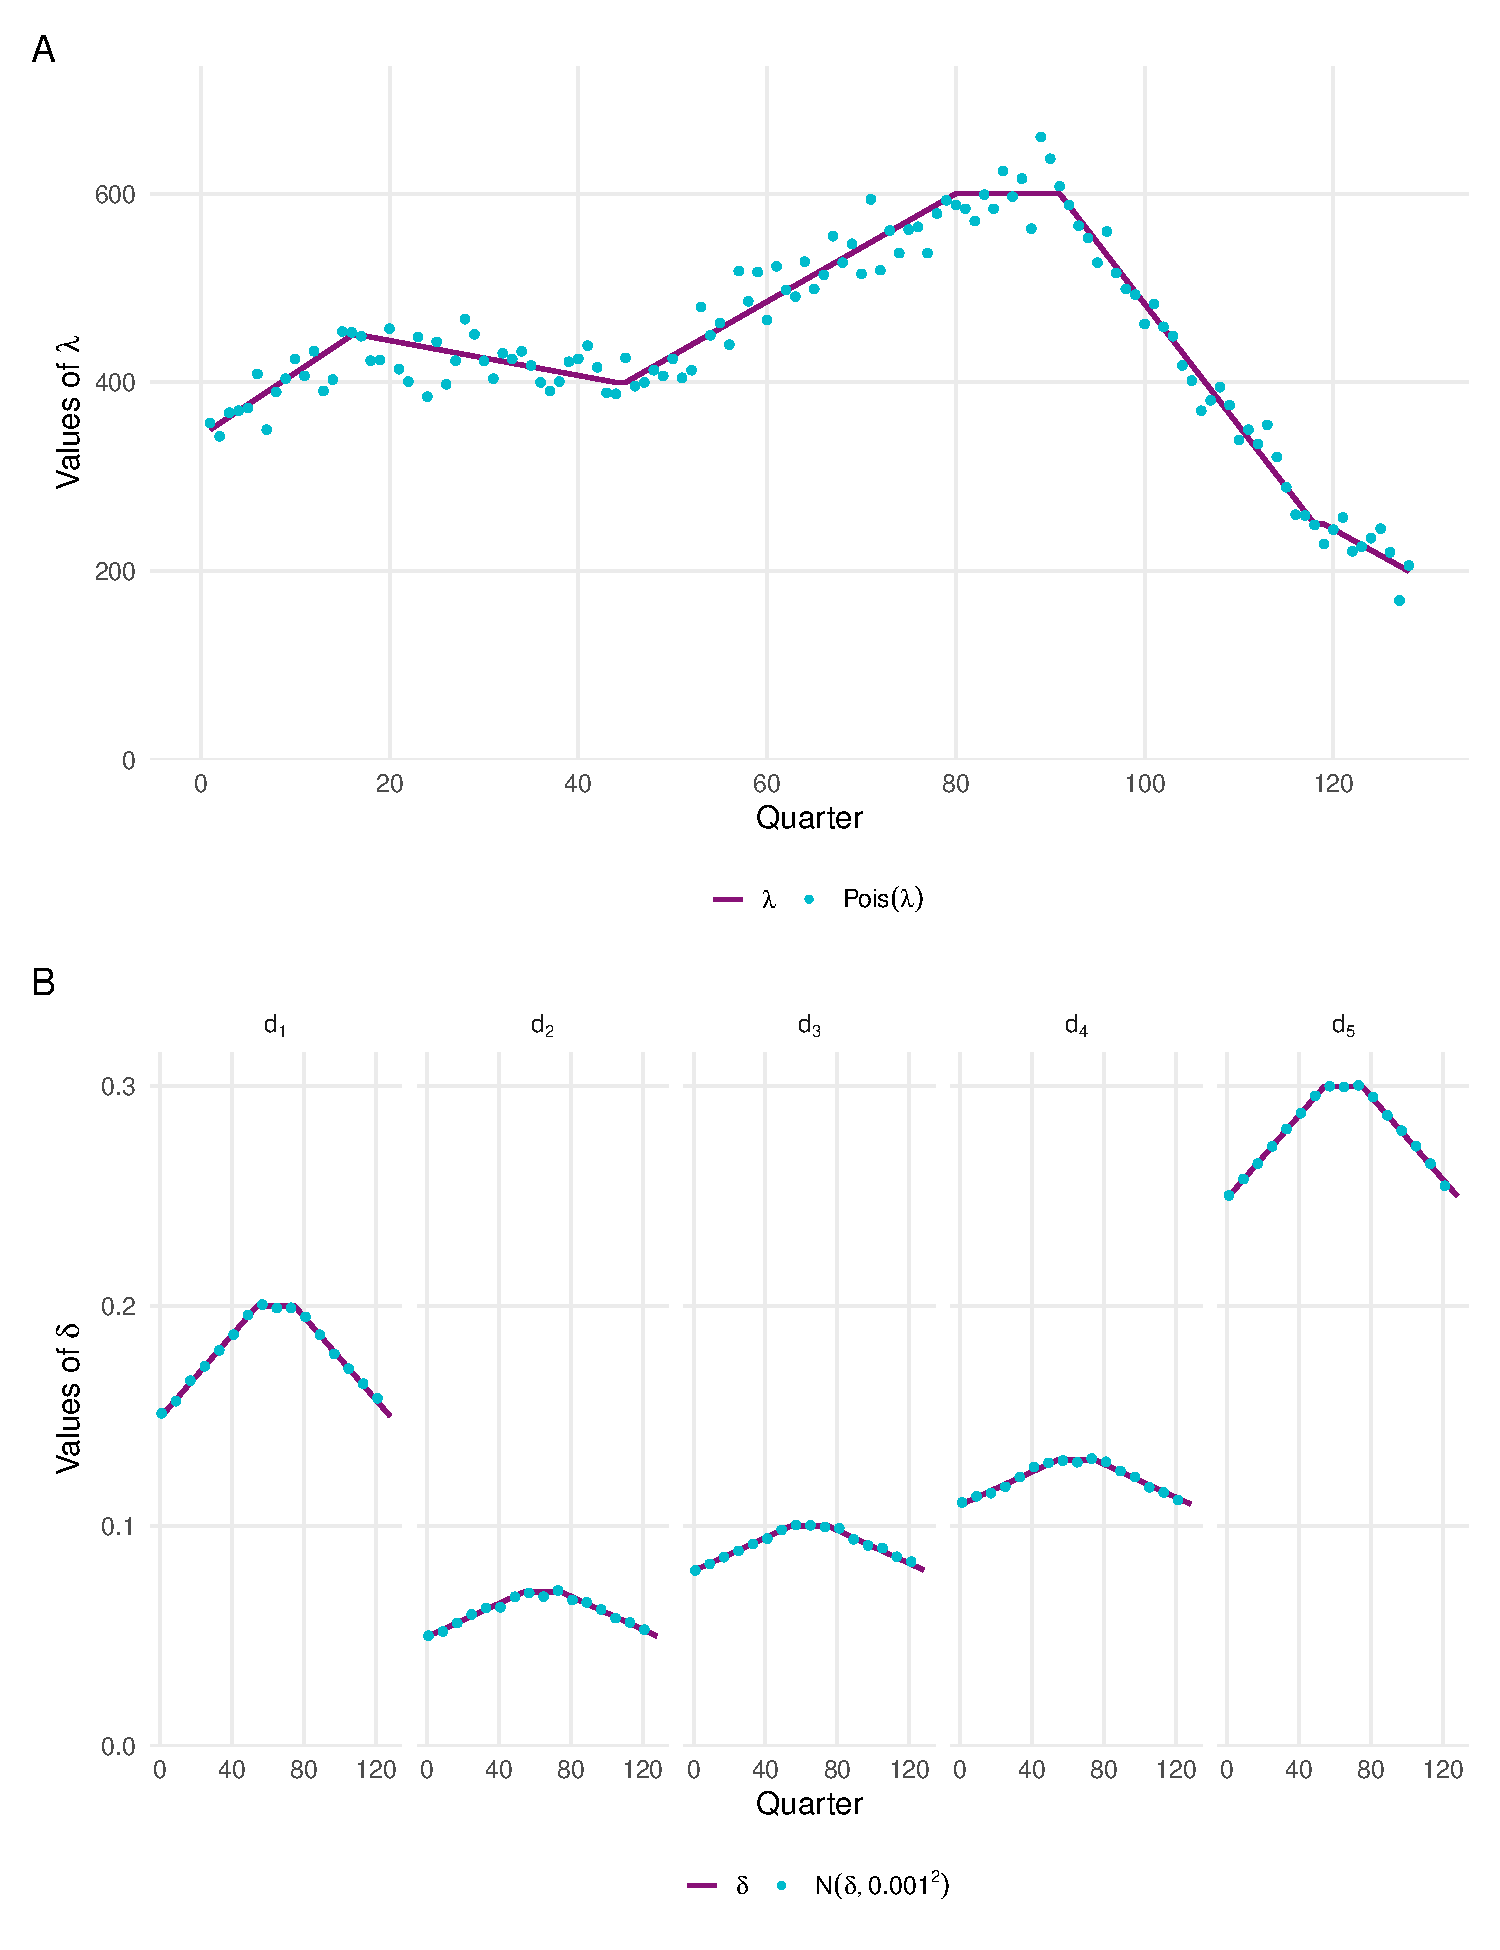
\includegraphics[width=\textwidth]{lambda_sim.pdf}
  \caption[Parameter values and sampled values of HIV incidence and HIV diagnosis probabilities from one sampling iteration]{Parameter values of $\lambda$ and sampled values of $\text{Pois}(\lambda)$ (panel A), and parameter values of $\delta$ and sampled values of $\text{N}(\delta, 0.001^2)$ (panel B) from one sampling iteration.}\label{fig:lambda_sim}
\end{figure}

The progression probabilities, $q_i$, were specified to be the same fixed probabilities of disease progression used for the back-calculation models. The initial prevalence in each latent state, $\bm{e}_0$, was specified as a multiple of the initial incidence simulated at time 0 ($h_0$), such that $\bm{e}_0= \{h_0, 0.8(h_0), 0.1(h_0), 4(h_0), 2(h_0), h_0, 0.25(h_0)\}$. For these simulated data the information on CD4 and RITA were assumed to be complete, both to reduce uncertainty in the model estimates and to aid comparison.

A total of 300 simulated datasets were obtained, using the dual biomarker model as the data generating process. Three model scenarios were constructed, shown below, using 100 datasets each. Each dataset included simulated values for $y^\text{H}_j$, $y^\text{A}_j$, $y^\text{R}_j$, and $y^\text{L}_{i,j}$. These values were sufficient for the dual-biomarker model (scenario (i)), but to fit the CD4-only back-calculation model (scenarios (ii) and (iii)) the requisite $y^\text{C}_j$ needed to be derived from combinations of these values.
%
\begin{enumerate}
  \item[(i)] No alteration of the simulated data:
        %
        \begin{itemize}
          \item the number of HIV and AIDS diagnoses over time were $y^\text{H}_j$ and $y^\text{A}_j$, respectively;
          \item the number of diagnoses over time with recently acquired HIV was $y^\text{R}_j$;
          \item the distribution of CD4 cell counts over time for those diagnosed with non-recent HIV was $y^\text{L}_{i,j}$;
        \end{itemize}

  \item[(ii)] Specifying a CD4 count distribution for recently acquired HIV diagnoses according to the distribution in Table~\ref{tab:cd4_dist_age}:
        %
        \begin{itemize}
          \item the number of HIV and AIDS diagnoses over time were $y^\text{H}_j$ and $y^\text{A}_j$, respectively;
          \item $y^\text{R}_{j}$ and $y^\text{L}_{i,j}$ were combined to derive an appropriate distribution of CD4 cell counts over time for all HIV diagnoses, $y^\text{C}_{i,j}$, according to:
                %
                \begin{align*}
                  y^\text{C}_{i,j} & = \rho_i y^\text{R}_{j} + y^\text{L}_{i,j} \\
                  \bm{\rho}        & = \{0.59, 0.27, 0.11, 0.03\}
                \end{align*}
        \end{itemize}

  \item[(iii)] Reclassifying all recently acquired HIV diagnoses to the 500+ CD4 stratum:
        %
        \begin{itemize}
          \item the number of HIV and AIDS diagnoses over time were $y^\text{H}_j$ and $y^\text{A}_j$, respectively;
          \item $y^\text{R}_{j}$ and $y^\text{L}_{i,j}$ were combined to derive an appropriate distribution of CD4 cell counts over time for all HIV diagnoses, $y^\text{C}_{i,j}$, according to:
                %
                \[
                  y^\text{C}_{i,j} =
                  \begin{dcases*}
                    y^\text{R}_{j} + y^\text{L}_{i,j} & for $i = 1$ \\
                    y^\text{L}_{i,j}                  & for $i > 1$
                  \end{dcases*}
                \]
        \end{itemize}

\end{enumerate}

\subsubsection{Estimands}

The estimands compared between the models were the posterior median and 95\% credible intervals of HIV incidence, HIV diagnosis probabilities, undiagnosed HIV prevalence, and the posterior predictive median and 95\% credible intervals for the number of HIV diagnoses.

\subsubsection{Methods}

Back-calculation models were fitted to the each of the simulated datasets to reconstruct the underlying HIV incidence and HIV diagnosis probabilities, with prior distributions as specified in earlier sections. The dual biomarker model was fitted to the datasets simulated in scenario (i), and the CD4-only model was fitted to the datasets simulated in scenarios (ii) and (iii). The specified estimands were generated by averaging over the posterior estimates from the 100 model fits in each scenario. Results for scenarios (i) and (ii) are shown below, with results for scenario (iii) included in Appendix~\ref{appendix:naivereclassify}

To investigate the effect of missing data, scenarios (i) and (ii) were re-simulated with the CD4 and RITA information missing for 40\% of diagnoses. The dual biomarker and CD4-only model were again fitted to these scenarios, results are included in Appendix~\ref{appendix:simmissing}.

Models were implemented in a Bayesian framework in the \texttt{R} and \texttt{STAN} software~\parencite{R_Core_Team2020-ca, Carpenter2017-wk}. Models were run with 4 chains for 2000 MCMC iterations each and inspection of trace plots and the $\hat{R}$ convergence statistics used to assess convergence~\parencite{Gelman1992-md}.

The bias and predictive mean squared error (PMSE)\nomenclature[z]{PMSE}{Predictive mean squared error} of the posterior mean HIV incidence were evaluated for each scenario. The bias is the expected difference between the parameter value specified for the data generating process, $\lambda_j$, and the estimated posterior mean incidence, $\hat{h}_{i,j}$, at each time point, $j = 1, \ldots, N$, over the 100 simulation iterations, $i = 1, \ldots, 100$:
%
\begin{align*}
  \text{Bias}(\hat{h}_j, \lambda_j) &= \frac{1}{100} \sum_{i=1}^{100} \hat{h}_{i,j} - \lambda_j
\end{align*}

The PMSE is the expectation of the squared differences over the 100 simulation iterations:
%
\[
  \text{PMSE}(\hat{h}) = \frac{1}{100} \frac{1}{N} \sum_{i=1}^{100} \sum_{j=1}^N{(\hat{h}_{i,j} - \lambda_{i,j})}^2
\]

where $N$ is the total number of simulated time points. A lower PMSE indicates that the parameter values are more accurately estimated. The bias and PMSE of the posterior mean HIV incidence are reported for each scenario, and the distribution of the differences and squared differences over the 100 simulations is shown.

\subsubsection{Performance measures}

Figure~\ref{fig:sim_estimates} panel A shows posterior HIV incidence estimates for the dual biomarker model and CD4-only model and fitted to scenarios (i) and (ii). Despite increased precision, the estimates from the dual biomarker model were somewhat more erratic.

\begin{figure}[htbp!]
  \centering
  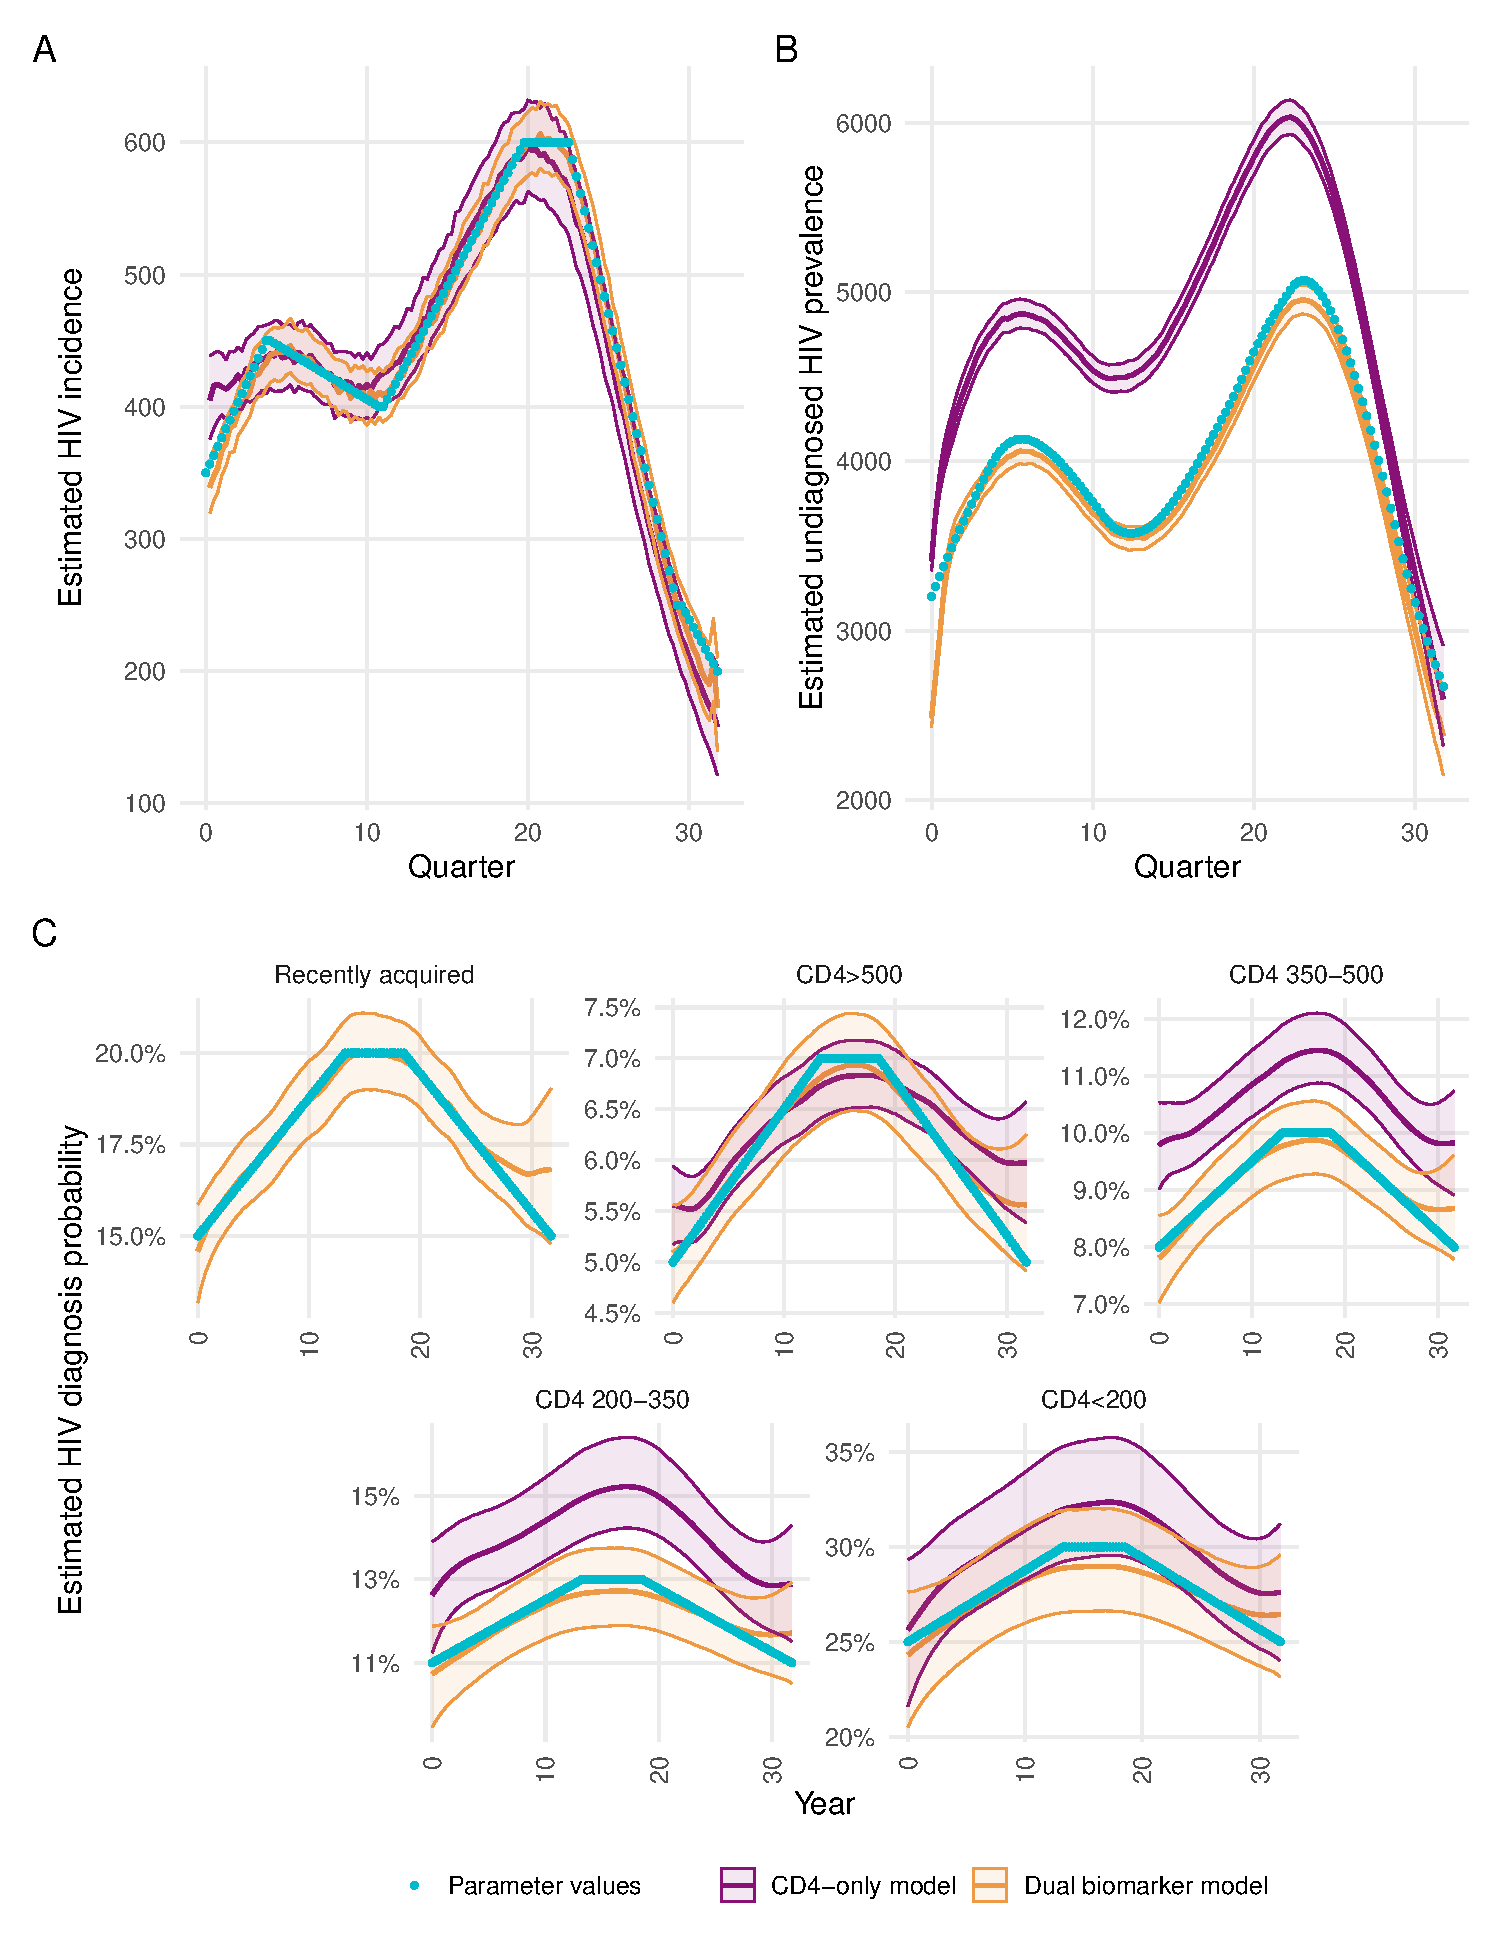
\includegraphics[width=\textwidth]{sim_estimates.pdf}
  \caption[Estimated posterior median and 95\% CrI of HIV incidence, undiagnosed prevalence, and diagnosis probabilities, by back-calculation model]{Estimated posterior median and 95\% CrI of HIV incidence (panel A), undiagnosed prevalence (panel B), and diagnosis probabilities (panel C), averaged over 100 model fits, compared to the specified parameter values, by back-calculation model.}\label{fig:sim_estimates}
\end{figure}

Both models were able to reconstruct the trend in undiagnosed HIV prevalence, as shown in Figure~\ref{fig:sim_estimates} panel B. However, the posterior estimates from the CD4-only model were a significant overestimate compared to the specified parameter values, which were better reconstructed by the dual biomarker model.

Both models reconstructed the trend in diagnosis probabilities, as shown in Figure~\ref{fig:sim_estimates} panel C. Whereas, the CD4-only model over-estimated the diagnosis probabilities in each strata, the dual biomarker model estimates were in line with the specified diagnosis probability parameter values.

Figure~\ref{fig:diag_fit_sim} shows the number of HIV diagnoses derived from the specified parameter values alongside the posterior predictive estimates from the CD4-only and dual biomarker models. For both models the predictive distributions fitted the data with comparable precision.

\begin{figure}[htbp!]
  \centering
  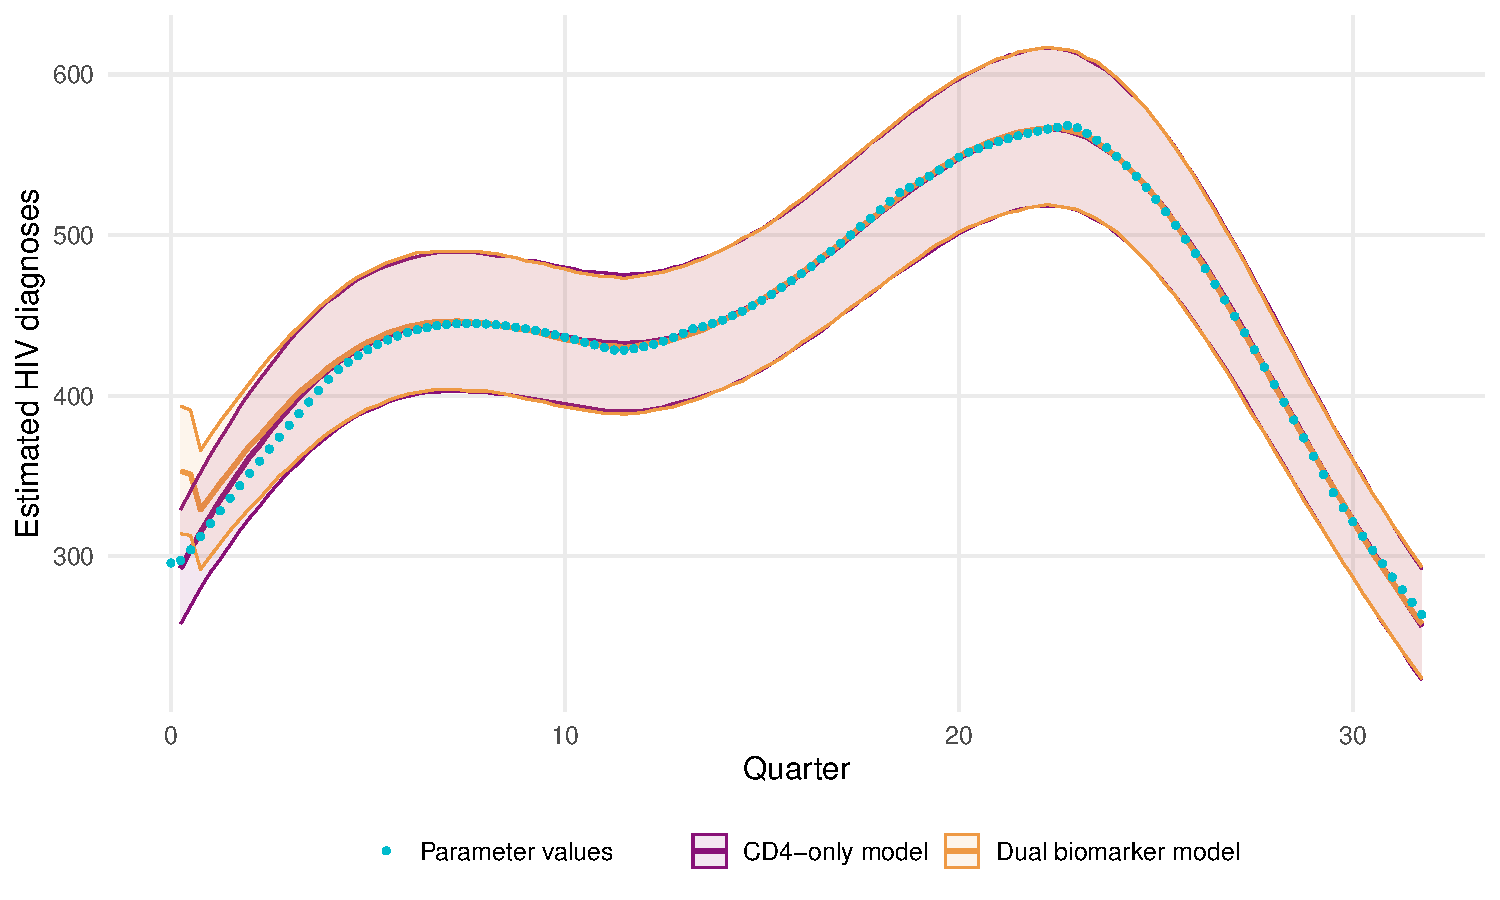
\includegraphics[width=\textwidth]{diag_fit_sim.pdf}
  \caption[Estimated HIV diagnoses (posterior predictive median and 95\% prediction interval), by back-calculation model]{Estimated HIV diagnoses (posterior predictive median and 95\% prediction interval) averaged over 100 model fits, compared to those derived from the specified parameter values, by back-calculation model.}\label{fig:diag_fit_sim}
\end{figure}

Figure~\ref{fig:mse_sim} panel A shows the distribution of differences and the bias for each model. On average, over the 100 model fits, there was smaller bias in the dual biomarker model (bias of -3.28) compared to the CD4-only model (bias of -4.48). Figure~\ref{fig:mse_sim} panel B shows the distribution of squared differences and PMSE for each model. The dual-biomarker model had a lower PMSE than the CD4-only model, 340.4 vs.\ 717.6, indicating a more accurate estimate of the parameter values.

\begin{figure}[htbp!]
  \centering
  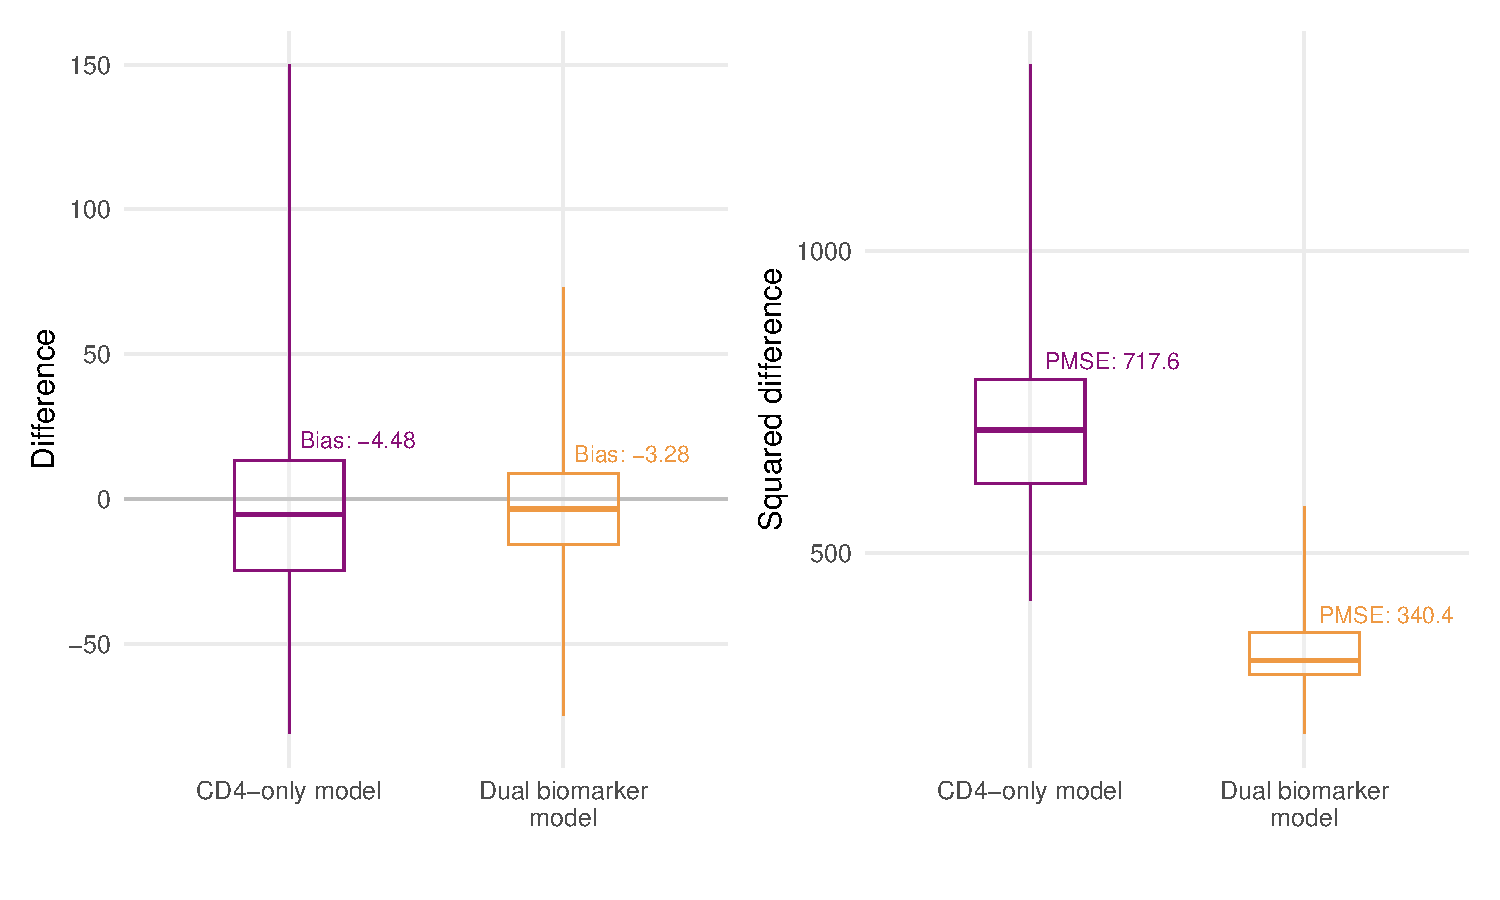
\includegraphics[width=\textwidth]{incidence_mse_sim.pdf}
  \caption[Distributions of differences and squared differences between parameter value and estimated HIV incidence, by back-calculation model]{Distributions of differences (panel A), and squared differences (panel B) between parameter value and estimated HIV incidence, by back-calculation model. Estimates from 100 model fits. Boxplots show median, inter-quartile range, and range of estimates for each model.}\label{fig:mse_sim}
\end{figure}

\begin{figure}[htbp!]
  \centering
  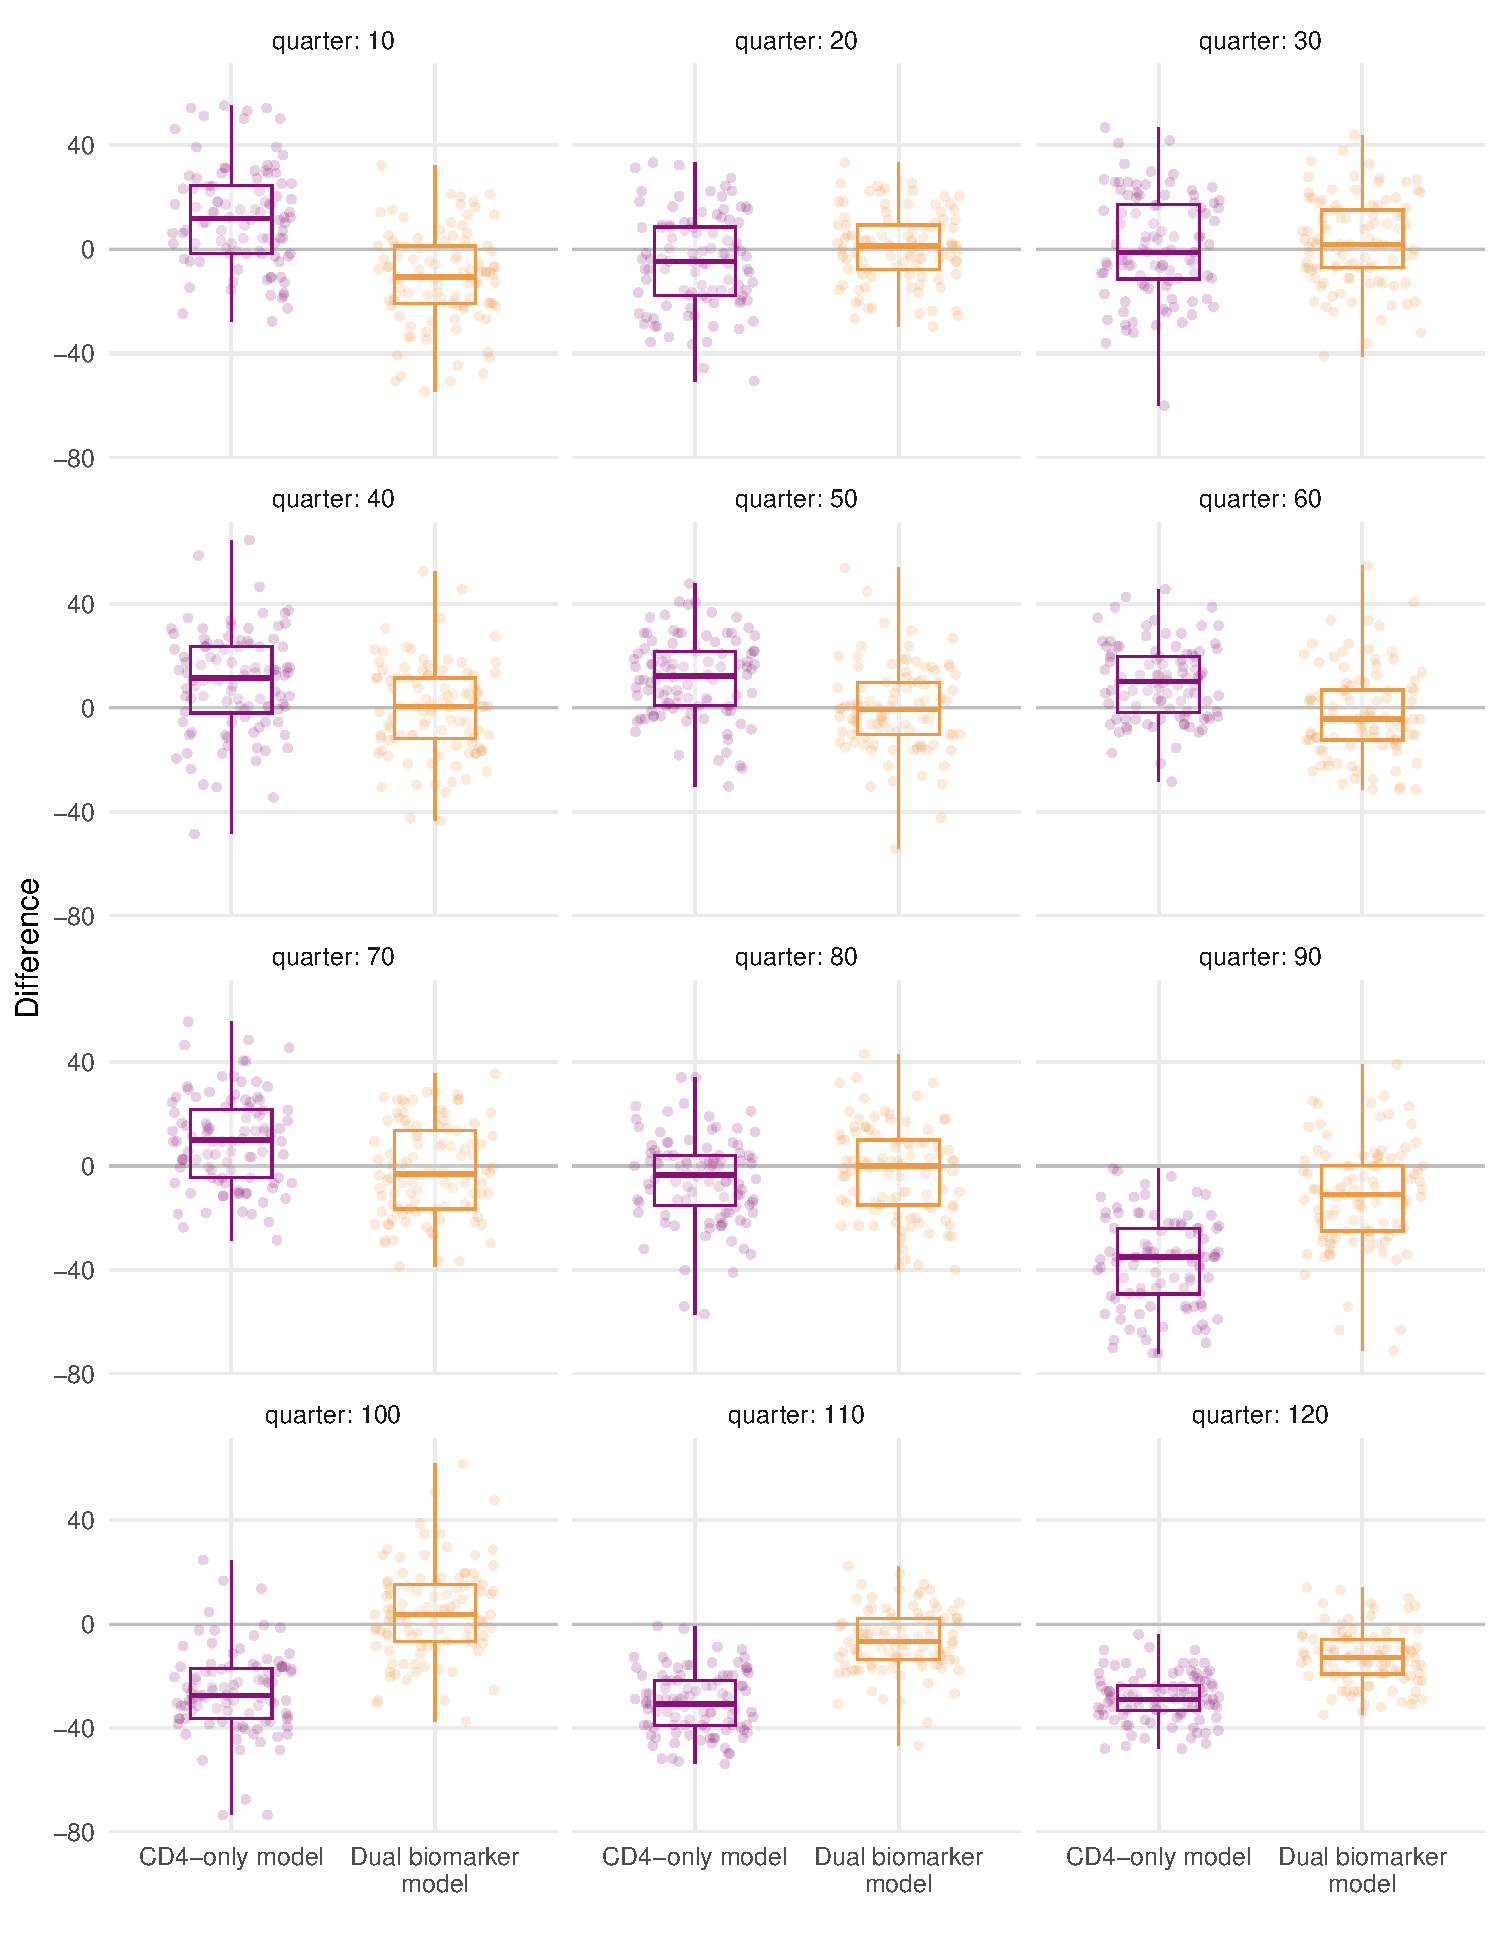
\includegraphics[width=\textwidth]{incidence_boxplot_sim_year.pdf}
  \caption[Distribution of differences between specified parameter value and estimated HIV incidence for selected quarters, by back-calculation model]{Distribution of differences between specified parameter value and estimated HIV incidence for selected quarters, by back-calculation model. Estimates from 100 model fits. Boxplots show median, inter-quartile range, and range of estimates for each model.}\label{fig:boxplot_sim_year}
\end{figure}

Figure~\ref{fig:boxplot_sim_year} shows the distribution of differences between the specified parameter value and the estimated HIV incidence for selected quarters, by model. The distributions varied by quarter, although the differences for the dual biomarker estimates tended to have smaller inter-quartile ranges.

\subsection{Application to national surveillance data}

The CD4-only and dual biomarker models were applied to HIV surveillance data for GBM newly diagnosed in England. As is standard practice, GBM born abroad and with a known prior diagnosis abroad were excluded from the analysis since they were unlikely to have been incident cases in England.

Figure~\ref{fig:rita_estimates} panel A shows posterior estimates of HIV incidence. Similar trends over time were estimated by both models, with slightly elevated median incidence between 2014--2017 in the CD4-only model. Estimates from the dual biomarker model had narrower 95\% credible intervals than the CD4-only model, and this continued up to the most recent quarter of data. For annual HIV incidence estimates, shown in Table~\ref{tab:incidence_annual}, again the dual biomarker model estimates had narrower 95\% credible intervals.

\begin{table}[!h]
\centering\centering
\caption{\label{tab:incidence_annual}Estimated annual incidence (posterior median and 95\% CrI) of HIV among GBM in EW\&NI between 2012--2019, by model.}
\centering
\begin{tabular}[t]{rll}
\toprule
\multicolumn{1}{c}{ } & \multicolumn{2}{c}{Model} \\
\cmidrule(l{3pt}r{3pt}){2-3}
  & CD4-only & Dual biomarker\\
\midrule
\addlinespace[0.3em]
\multicolumn{3}{l}{Year}\\
\hspace{1em}2012 & 2540 (2280, 2960) & 2400 (2180, 2640)\\
\hspace{1em}2013 & 2740 (2360, 3130) & 2570 (2320, 2850)\\
\hspace{1em}2014 & 2270 (1980, 2570) & 2410 (2200, 2700)\\
\hspace{1em}2015 & 1670 (1380, 1940) & 1900 (1640, 2140)\\
\hspace{1em}2016 & 1300 (1030, 1600) & 1560 (1340, 1800)\\
\hspace{1em}2017 & 1150 (900, 1440) & 1290 (1070, 1580)\\
\hspace{1em}2018 & 1070 (760, 1440) & 1060 (810, 1410)\\
\hspace{1em}2019 & 1020 (540, 1790) & 960 (630, 1570)\\
\bottomrule
\end{tabular}
\end{table}


\begin{figure}[htbp!]
  \centering
  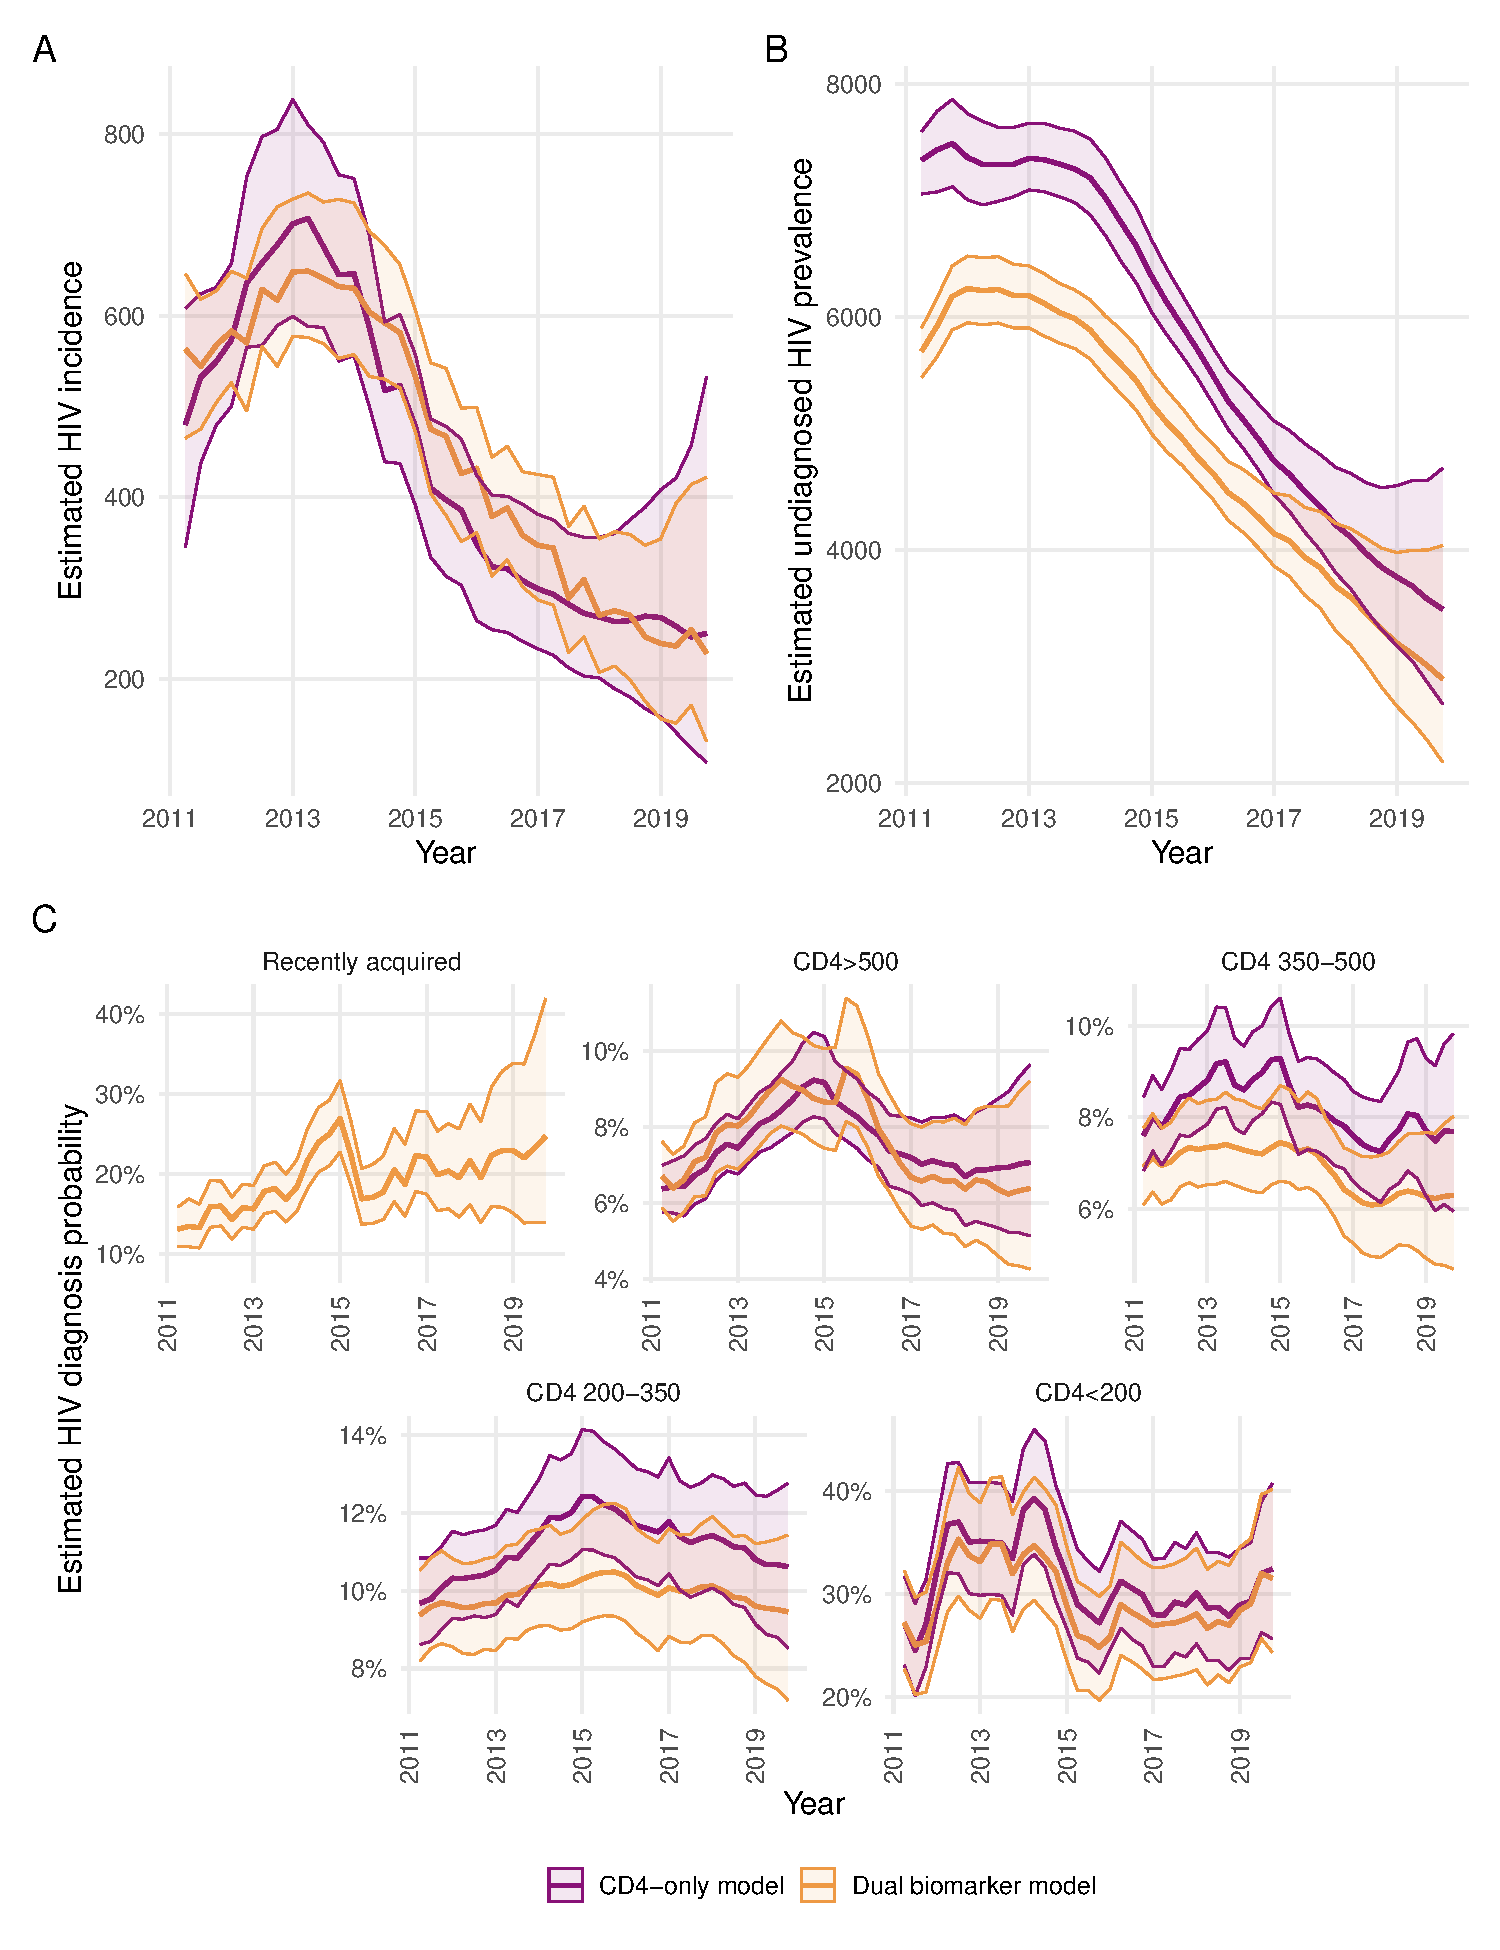
\includegraphics[width=\textwidth]{rita_estimates.pdf}
  \caption[Estimated posterior median and 95\% CrI of HIV incidence, undiagnosed prevalence, and diagnosis probabilities for GBM diagnosed in England, 2011--2019]{Estimated posterior median and 95\% CrI of HIV incidence (panel A), undiagnosed prevalence (panel B), and diagnosis probabilities (panel C) fitted to HIV diagnosis data for GBM diagnosed in England, 2011--2019.}\label{fig:rita_estimates}
\end{figure}

Undiagnosed HIV prevalence estimates from the dual biomarker model were significantly lower than those estimated by the CD4-only model for the years 2011--2017, with some overlap in more recent years (Figure~\ref{fig:rita_estimates} panel B). Meanwhile, HIV diagnosis probability estimates were broadly similar for both models across most CD4 strata, with additional information about recently acquired infections from the dual biomarker model (Figure~\ref{fig:rita_estimates} panel C).

Figure~\ref{fig:diag_fit_rita} shows that both models were a good fit to the observed diagnosis data, with the 95\% predictive intervals containing almost all of the data points.

\begin{figure}[htbp!]
  \centering
  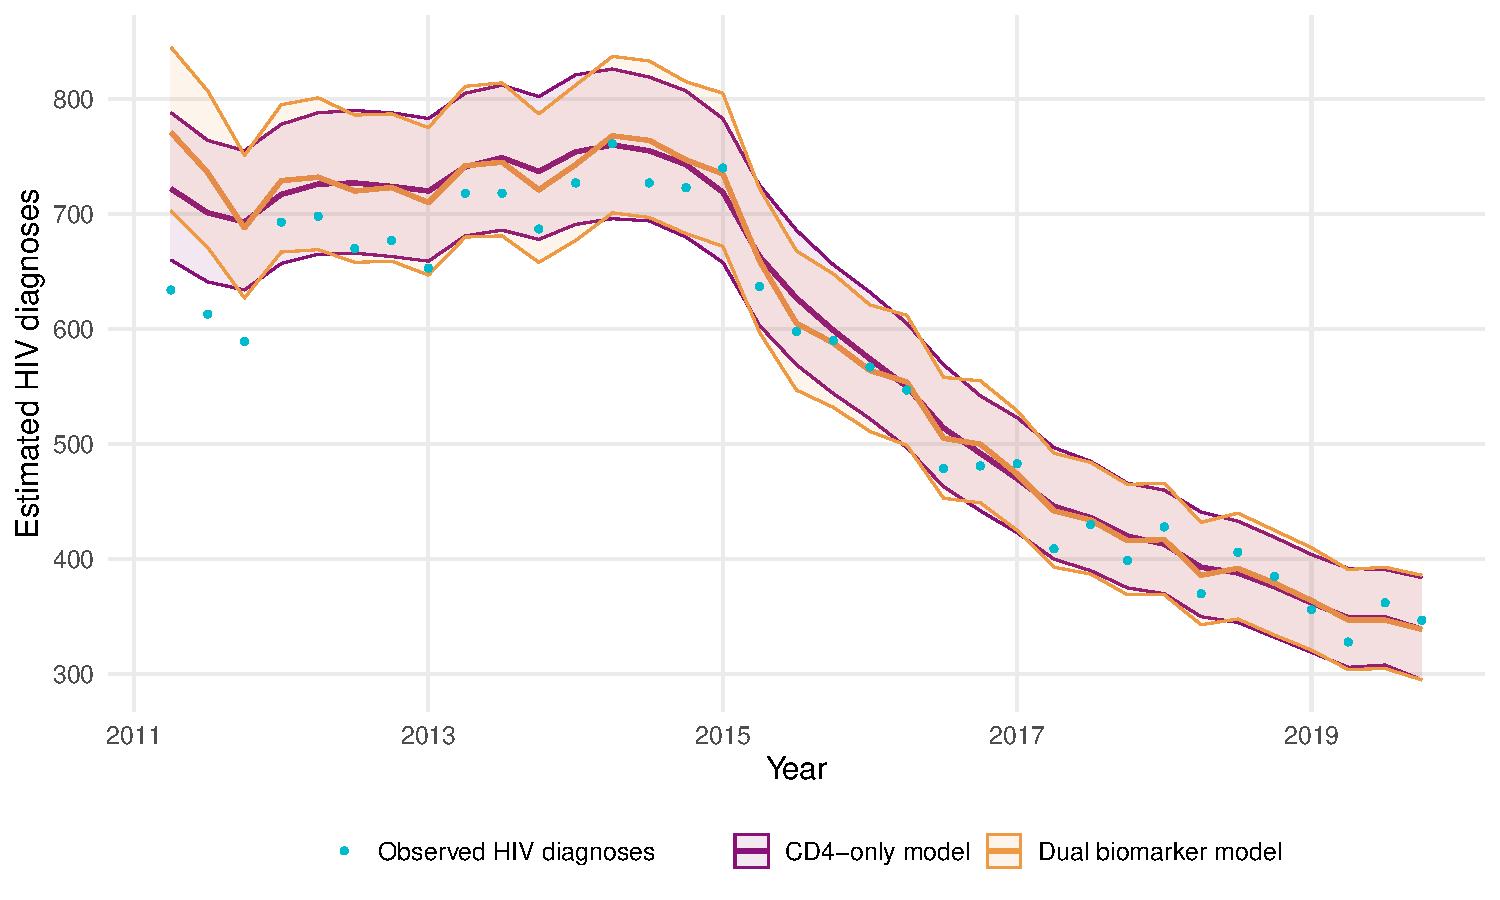
\includegraphics[width=\textwidth]{diag_fit_rita.pdf}
  \caption[Estimated HIV diagnoses (posterior predictive median and 95\% prediction interval) for GBM diagnosed in England, 2011--2019]{Estimated HIV diagnoses (posterior predictive median and 95\% prediction interval), compared to observed HIV diagnosis data for GBM diagnosed in England, 2011--2019.}\label{fig:diag_fit_rita}
\end{figure}

\subsection{Conclusions}

The CD4-only and dual biomarker model were used to reconstruct trends in HIV incidence, undiagnosed prevalence, probability of diagnosis, and quarterly numbers of diagnoses for simulated scenarios and real-world surveillance data.

In the simulation study, all relevant estimates from the dual biomarker model were in-line with the specified parameter values, and accurate trends could be inferred from the estimates. The CD4-only model gave accurate, although somewhat less precise, estimates of HIV incidence, but over-estimated the HIV diagnosis probabilities and undiagnosed HIV prevalence as compared to the specified parameter values. This lack of fit of the CD4-only model is not surprising, since the model does not account for diagnosis during the acute stage.

Estimates of HIV incidence, the key quantity of interest in current back-calculation models, were similar for both models. However, the dual biomarker model estimates were closer to the simulated values on average, and estimated with greater precision.

By applying these models to surveillance data for GBM newly diagnosed in England, trends could be estimated for unobserved quantities. As for the simulation study, whilst trends were similar in both models, the dual biomarker model gave more precise estimates of HIV incidence and a significantly lower estimate of undiagnosed HIV prevalence before 2017. Based on the simulation study, and knowing that diagnosis occurring during the acute and seroconversion phases can lead to low CD4 counts, the estimates from the dual biomarker model are likely to be more accurate estimates of these unobserved quantities.

Whilst comparison of these estimates with a `true' unobserved quantity is not possible for real-world data, the back-calculation estimates can be compared with estimates obtained via different methods. The MPES model has provided estimates of undiagnosed HIV prevalence among GBM in England since 2013~\parencite{Presanis2021-pv}. As shown in Figure~\ref{fig:undiag_prev_mpes}, undiagnosed prevalence estimates from both the CD4-only and dual biomarker back-calculation models fall within the 95\% credible interval from MPES, with the median MPES estimate being closer to the dual biomarker model, especially in more recent years. The wider credible range in MPES compared to the back-calculation reflects uncertainty in several of the MPES data sources which are not considered in the back-calculation model.

\begin{figure}[htbp!]
  \centering
  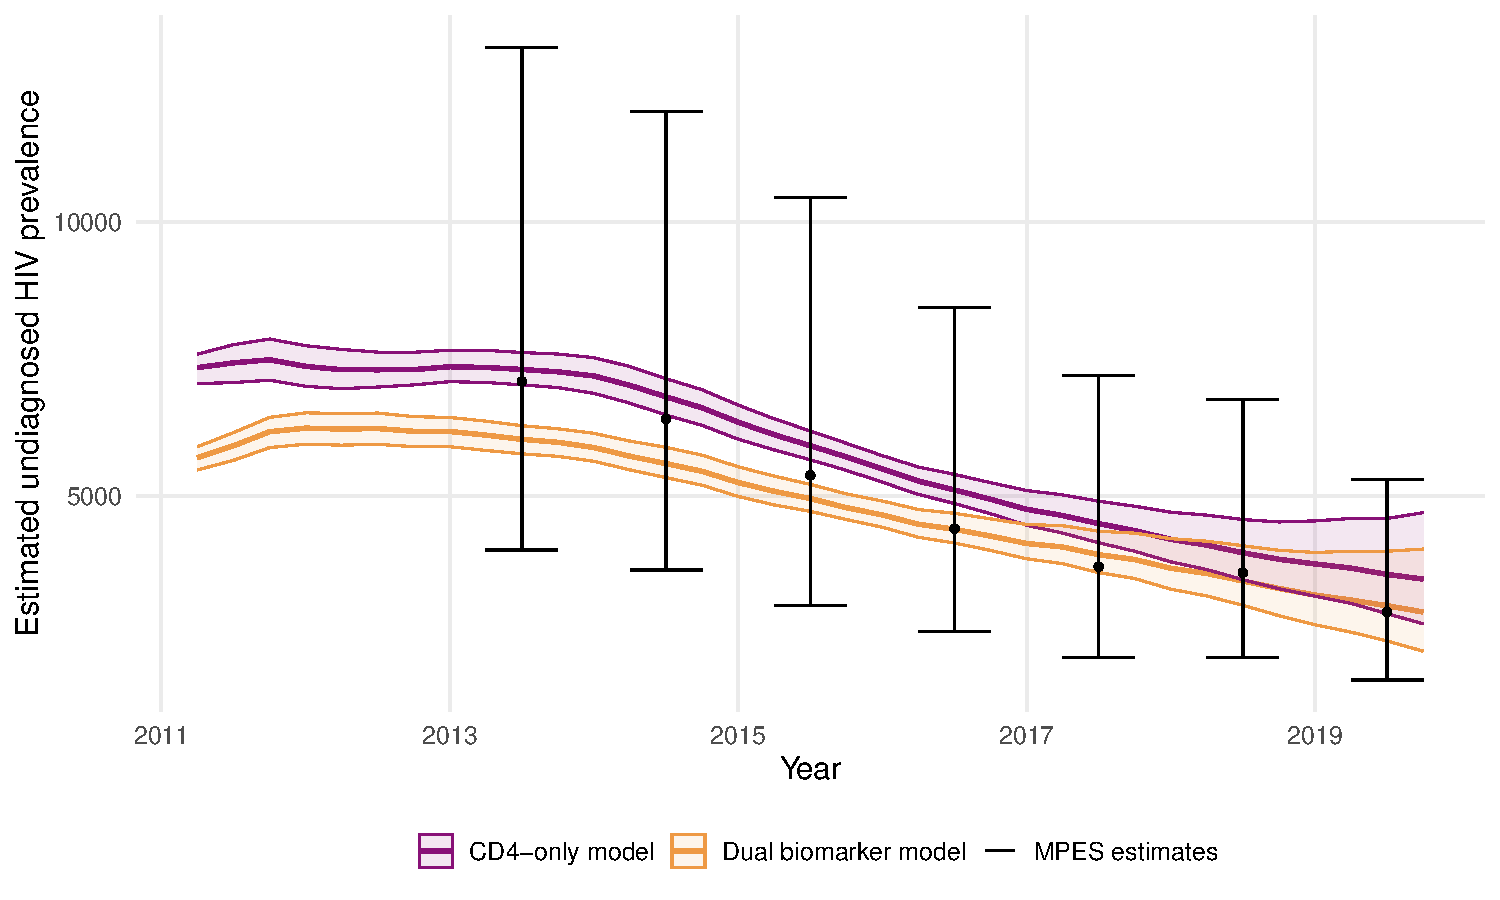
\includegraphics[width=\textwidth]{undiag_prev_mpes.pdf}
  \caption[Estimated undiagnosed HIV prevalence (posterior median and 95\% CrI) from dual biomarker and CD4-only back-calculation, compared to MPES estimates for GBM diagnosed in England, 2011--2019]{Estimated undiagnosed HIV prevalence (posterior median and 95\% CrI) from dual biomarker and CD4-only back-calculation, compared to MPES estimates for GBM diagnosed in England, 2011--2019.}\label{fig:undiag_prev_mpes}
\end{figure}

In addition to improved estimate precision and accuracy, the dual biomarker model provides additional information on the probability of diagnosis among individuals with recently acquired HIV\@. These estimates are of interest for epidemiologists as trends can be correlated with HIV prevention programmes. In the English estimates for 2011--2019, there was a spike in the probability of being recently diagnosed during 2015, followed by a slower rise to the end of 2019. The 2015 spike coincides with a rapid increase in testing and in diagnoses of recently acquired HIV at a major combined sexual health and HIV service in an area of central London known for its high concentration of LGBTQI venues~\parencite{Girometti2021-cp}.

Unsurprisingly, given the small value of the progression probability $q_1$, a simple reclassification of recent diagnoses shown in Appendix~\ref{appendix:naivereclassify} yielded very similar estimates to the dual biomarker model, with minimal loss of precision. The dual biomarker model remains the more accurate method to incorporate additional biomarker data, reflecting the 6-month MDRI and providing valuable information about HIV diagnosis probability in the early infection period.

\subsubsection{Limitations}

The methodology presented here makes use of a single biomarker classification (recent/non-recent infection) although does not address false recency error in this classification, which was previously estimated as 1.9\% (95\% CI 1.0--3.4\%)~\parencite{Aghaizu2018-kk}. Accounting for this error may lessen the change in undiagnosed HIV prevalence, although the difference is likely to be small.

As previously noted, there were regional differences in the availability of HIV avidity information, with particularly low availability in Wales. HIV testing policies also vary between different devolved nations which results in differences in the proportion of recent diagnoses~\parencite{Kirwan2022-za}. To mitigate these regional biases, and for consistency with the HIV action plan for England and HIV estimation methods applied annually~\parencite{Department-of-Health-and-Social-Care2021-ee, Martin2023-um}, the models were applied only to surveillance data for England. There was also observed to be some age-dependency in the availability of the recency assay data which was not accounted for. Whilst the effect on the model estimates is likely to be small, development of the age-dependent back-calculation model to include avidity information may help to more formally address this potential bias.

GBM diagnosed with HIV in England are an increasingly diverse group, with 34\% of those newly diagnosed in 2022 born abroad and potentially having acquired HIV outside of England~\parencite{Martin2023-um}. However, a limitation of all currently existing models is the assumption of a closed system which does not account for external processes such as immigration and emigration. Currently this is addressed by excluding GBM born abroad and first diagnosed outside of the UK from the diagnosis dataset. However, the method remains unsuited for use among heterosexual groups due to the large proportion born abroad, and may become unreliable as the GBM population becomes increasingly diverse.

This chapter has developed the CD4 back-calculation model into a dual biomarker model, taking account of biases in the data and improving the precision and accuracy of HIV incidence estimates for England. Avenues for further development, for example including age-specific back-calculation and the incorporation of migration data are discussed further in Chapter~\ref{cha:conclusions}.

\section{Impact of COVID-19 lockdown on HIV}

\subsection{Background}

The analyses in this chapter have so far considered HIV diagnosis data prior to 2020. In 2020 the epidemiology of many infectious diseases was severely affected by the COVID-19 pandemic, with changes to healthcare services and so-called `lockdown' strategies and other measures being implemented worldwide to control the spread of COVID-19~\parencite{Institute_for_Government2022-zw}. The emergency response to COVID-19 likely impacted transmission (due to restrictions on social mixing) and testing activity (due to services being reconfigured and people being less able to access testing) for a multitude of non-COVID-related infectious diseases~\parencite{Mude2023-ec, Simoes2020-ri}. Whilst healthcare access and social mixing have now largely returned to pre-pandemic levels, understanding the effect of an abrupt change in testing and diagnosis for other conditions requires further research.

One concern is that existing methodologies which rely on time-series data to uncover trends in infectious disease may not be sufficiently sensitive to account for such sudden changes, or may incorrectly attribute their cause. Other analyses of English HIV diagnosis data, using a synthetically-controlled Bayesian structural time series model to infer the causal impact of the first lockdown in England, estimated 51 missed diagnoses (95\% prediction interval -310--393) among GBM during 2020~\parencite{Muhammed2024-dw}. However, the sensitivity of the back-calculation estimates to this drop and to different assumptions about the effect of COVID-19 lockdown is so far untested.

Estimating the specific impact of COVID-19 mitigation on HIV and other infectious diseases is important for re-evaluation of public health priorities post-pandemic. The public health response to COVID-19 diverted efforts away from England's HIV elimination agenda. Assessing if England remains on-target to eliminate HIV transmission by 2030 (as was previously estimated using the CD4 back-calculation~\parencite{Brizzi2021-zl}), or if further investment is required (as has been recently suggested by a stochastic simulation-based approach~\parencite{Cambiano2023-lj}), is vital to inform ongoing HIV prevention efforts.

\subsection{Aims}

This section aims to assess the sensitivity of HIV estimates for 2020 and 2021 to different lockdown effect assumptions, to evaluate the impact of COVID-19 on HIV incidence, and to assess if England remains on track to eliminate HIV as a public health threat by 2030. While not a formal causal inference study, similar sensitivity or stochastic scenario analyses have been conducted for influenza as a type of `counterfactual' analysis~\parencite{Wu2017-ts, Cooper2006-nl}.

\subsection{COVID-19 lockdown effect assumptions}

\subsubsection{Data}

The HIV surveillance data used in these analyses relate to GBM first diagnosed in England, with GBM born abroad and with a known prior diagnosis abroad being excluded.

This analysis considers changes in HIV transmission and probability of diagnosis during the 2-year period post-lockdown. Information on the timing of national and local COVID-19 lockdowns in England were available from the Institute for Government~\parencite{Institute_for_Government2022-zw}. Legal COVID-19 lockdown measures instructing people to stay at home were introduced in England on 26 March 2020, i.e.\ around the start of the second calendar quarter of 2020 (2020Q2).

Figure~\ref{fig:lockdown_diagnoses} shows quarterly HIV diagnoses among GBM in England before and after lockdown restrictions were introduced. A reduction in the number of new HIV diagnoses was particularly apparent during 2020Q2 (April to June) and 2020Q3 (July to September). Diagnoses recovered somewhat during 2020Q4 (October to December) and 2021Q1 (January to March), but were lower again during 2021Q2 to 2021Q4.

\begin{figure}[htbp!]
  \centering
  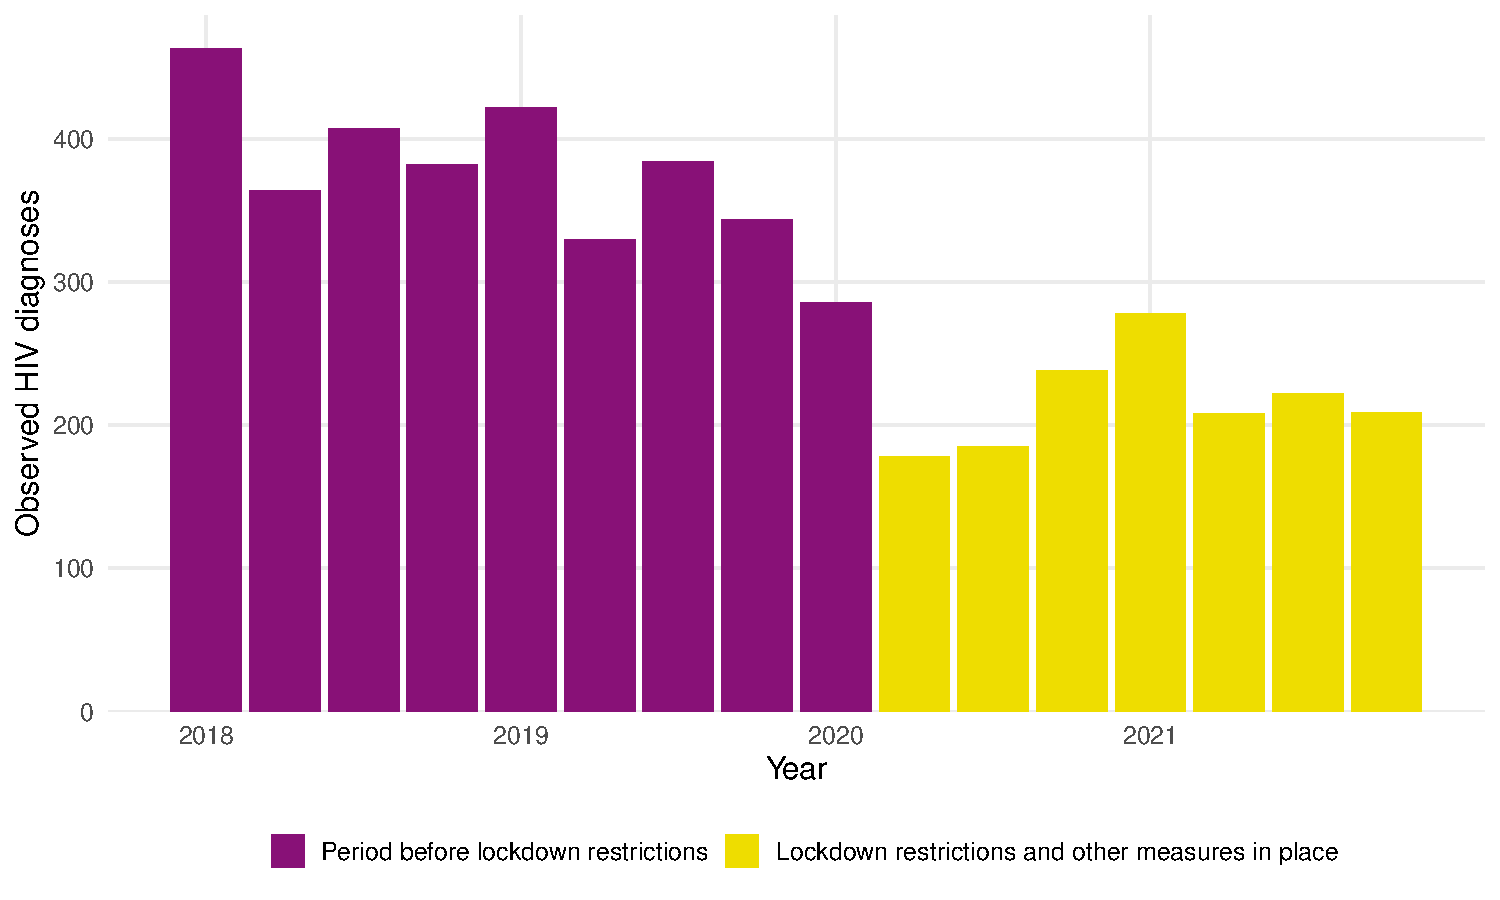
\includegraphics[width=\textwidth]{lockdown_diagnoses.pdf}
  \caption[Quarterly number of HIV diagnoses among GBM diagnosed in England, before and after introduction of lockdown restrictions, 2018--2021]{Quarterly number of HIV diagnoses among GBM diagnosed in England, before and after introduction of lockdown restrictions, 2018--2021.}\label{fig:lockdown_diagnoses}
\end{figure}

\subsubsection{Methods}

Observed HIV and AIDS diagnoses in the CD4 back-calculation are modelled as realisations of thinned Poisson processes from an unobserved, time-varying, incidence process, $h_j$. Expected HIV and AIDS diagnoses, $\mu_{i,j}$, are related to this incidence process via prevalent latent infections, $e_{i,j}$, known disease progression probabilities, $q_i$, and estimated diagnosis probabilities, $d_{i,j}$. Figure~\ref{fig:counterfactdag} shows the relationship between underlying HIV infections, HIV diagnosis probabilities, and HIV diagnoses in a schematic diagram.

\begin{figure}[htbp!]
  \centering
  \begin{tikzpicture}
    \SetGraphUnit{2}
    \Vertex[Math, L = h_j,x=0,y=2]{h}
    \Vertex[Math, L = d_{i,j},x=2,y=2]{d}
    \Vertex[Math, L = \mu_{i,j},x=1,y=0]{u}
    %\Vertex[Math, L = e_{i,j},x=0,y=0]{e}
    \Edges(h, u)
    \Edges(d, u)
    %\Edges(h, e) 
    %\Edges(d, e)
  \end{tikzpicture}
  \caption[Schematic diagram linking HIV infections and HIV diagnosis probabilities to HIV diagnoses]{Schematic diagram linking HIV infections $h_j$ and HIV diagnosis probabilities $d_{i,j}$ to HIV diagnoses $\mu_{i,j}$.}\label{fig:counterfactdag}
\end{figure}

In the CD4 back-calculation model, estimates of the contributions of the unknown incidence ($h_j$) and diagnosis probability ($d_{i,j}$) parameters to the expected diagnoses depend on all of:\ the diagnosis data, the CD4 count data, the prior distributions (including point priors) on the progression rates ($q$), and the incidence and diagnosis probabilities themselves. To assess the sensitivity of the estimates to different assumptions about the effect of lockdowns on the $h_j$ and $d_{i,j}$ parameters, the model can be modified with additional prior information about $h_j$ and $d_{i,j}$.

Three model scenarios were considered:
%
\begin{enumerate}
  \item[-] the unmodified model, with any disruption in diagnosis data taken at face-value and apportioned to the $h_j$ and $d_{i,j}$ parameters.

  \item[(a)] a scenario where the incidence of HIV was unaffected by the lockdowns and remained the same as in 2019, whereas probability of HIV diagnosis was allowed to be affected. In this scenario, the prior for $h_j$ in the calendar quarters $j \in \{2020\text{Q}2,\dots, 2021\text{Q}4\}$ was specified as $h_j \sim \text{Poisson}(\lambda_{2019\text{Q}k})$, where $\lambda_{2019\text{Q}k}$ is the HIV incidence in the $k$th quarter of 2019. This approximated HIV incidence in 2020 and 2021 remaining at the same level as 2019.

  \item[(b)] a scenario where the probability of HIV diagnosis was unaffected by the lockdowns and remained unchanged from 2019, whereas incidence was allowed to be affected. In this scenario, the prior for $d_{i,j}$ in the calendar quarters $j \in \{2020\text{Q}2,\dots, 2021\text{Q}4\}$ was specified as $d_{i,j} \sim \text{N}(\mu_{i,2019\text{Q}k}, 0.001^2)$, where $\mu_{i,2019\text{Q}k}$ is the diagnosis probability in the $i$th CD4 stratum and $k$th quarter of 2019. This approximated the probability of diagnosis in 2020 and 2021 in each CD4 stratum remaining at the same level as 2019.
\end{enumerate}

The unmodified model and scenarios (a) and (b) were each fitted to the observed HIV diagnosis data for GBM newly diagnosed in England between 2011--2021. Models were run with 4 chains and for 4000 MCMC iterations, with inspection of trace plots and the $\hat{R}$ convergence statistics used to assess convergence~\parencite{Gelman1992-md}.

Visual comparison and leave-one-out cross-validation (LOO-CV) using Pareto smoothed importance sampling were used to compare models~\parencite{Vehtari2024-qb}. The LOO Information Criterion (LOOIC) is similar to the frequentist Akaike information criterion (AIC), and enables the `best fitting' model to be identified whilst balancing parsimony and over-fitting.

\subsubsection{Results}

Figure~\ref{fig:counterfactual_estimates} panels A and B show a downwards trend in estimated HIV incidence between 2016--2021 in both the unmodified model and scenario (a) (where HIV incidence was assumed unaffected by lockdown), with estimates being more precise in scenario (a). The incidence estimates in scenario (b) (where diagnosis probabilities were assumed to be unaffected by lockdown) were more uncertain, but a similar downwards trend in incidence was estimated.

During 2020 and 2021 the 95\% credible intervals of annual incidence for all scenarios overlapped, with the posterior median being lowest in scenario (b) (Table~\ref{tab:counterfactual_inc_annual}).

\begin{table}[!h]
\centering\centering
\caption{\label{tab:counterfactual_inc_annual}Estimated annual incidence (posterior median and 95\% CrI) of HIV among GBM in EW\&NI between 2012--2021, by model.}
\centering
\begin{tabular}[t]{rlll}
\toprule
\multicolumn{1}{c}{ } & \multicolumn{3}{c}{Scenario} \\
\cmidrule(l{3pt}r{3pt}){2-4}
  & Unmodified model & (a) Incidence unaffected & \makecell[l]{(b) Diagnosis probabilities\\unaffected}\\
\midrule
\addlinespace[0.3em]
\multicolumn{4}{l}{Year}\\
\hspace{1em}2016 & 1420 (1290, 1560) & 1430 (1300, 1530) & 1310 (1140, 1500)\\
\hspace{1em}2017 & 1090 (960, 1210) & 1080 (980, 1180) & 950 (780, 1160)\\
\hspace{1em}2018 & 860 (720, 1030) & 740 (660, 820) & 770 (570, 1020)\\
\hspace{1em}2019 & 650 (490, 840) & 550 (500, 610) & 530 (330, 830)\\
\hspace{1em}2020 & 530 (360, 780) & 460 (380, 530) & 370 (180, 790)\\
\hspace{1em}2021 & 410 (210, 830) & 360 (250, 480) & 260 (80, 890)\\
\bottomrule
\end{tabular}
\end{table}


HIV diagnosis probabilities in the unmodified model and in scenario (a) showed high sensitivity to the impact of COVID-19 lockdowns, with a reduction in the probability of diagnosis being observed across all CD4 strata (Figure~\ref{fig:counterfactual_estimates} panels C and D). In scenario (b) the diagnosis probabilities were more stable (by design), but particularly uncertain after 2019.

\begin{figure}[htbp!]
  \centering
  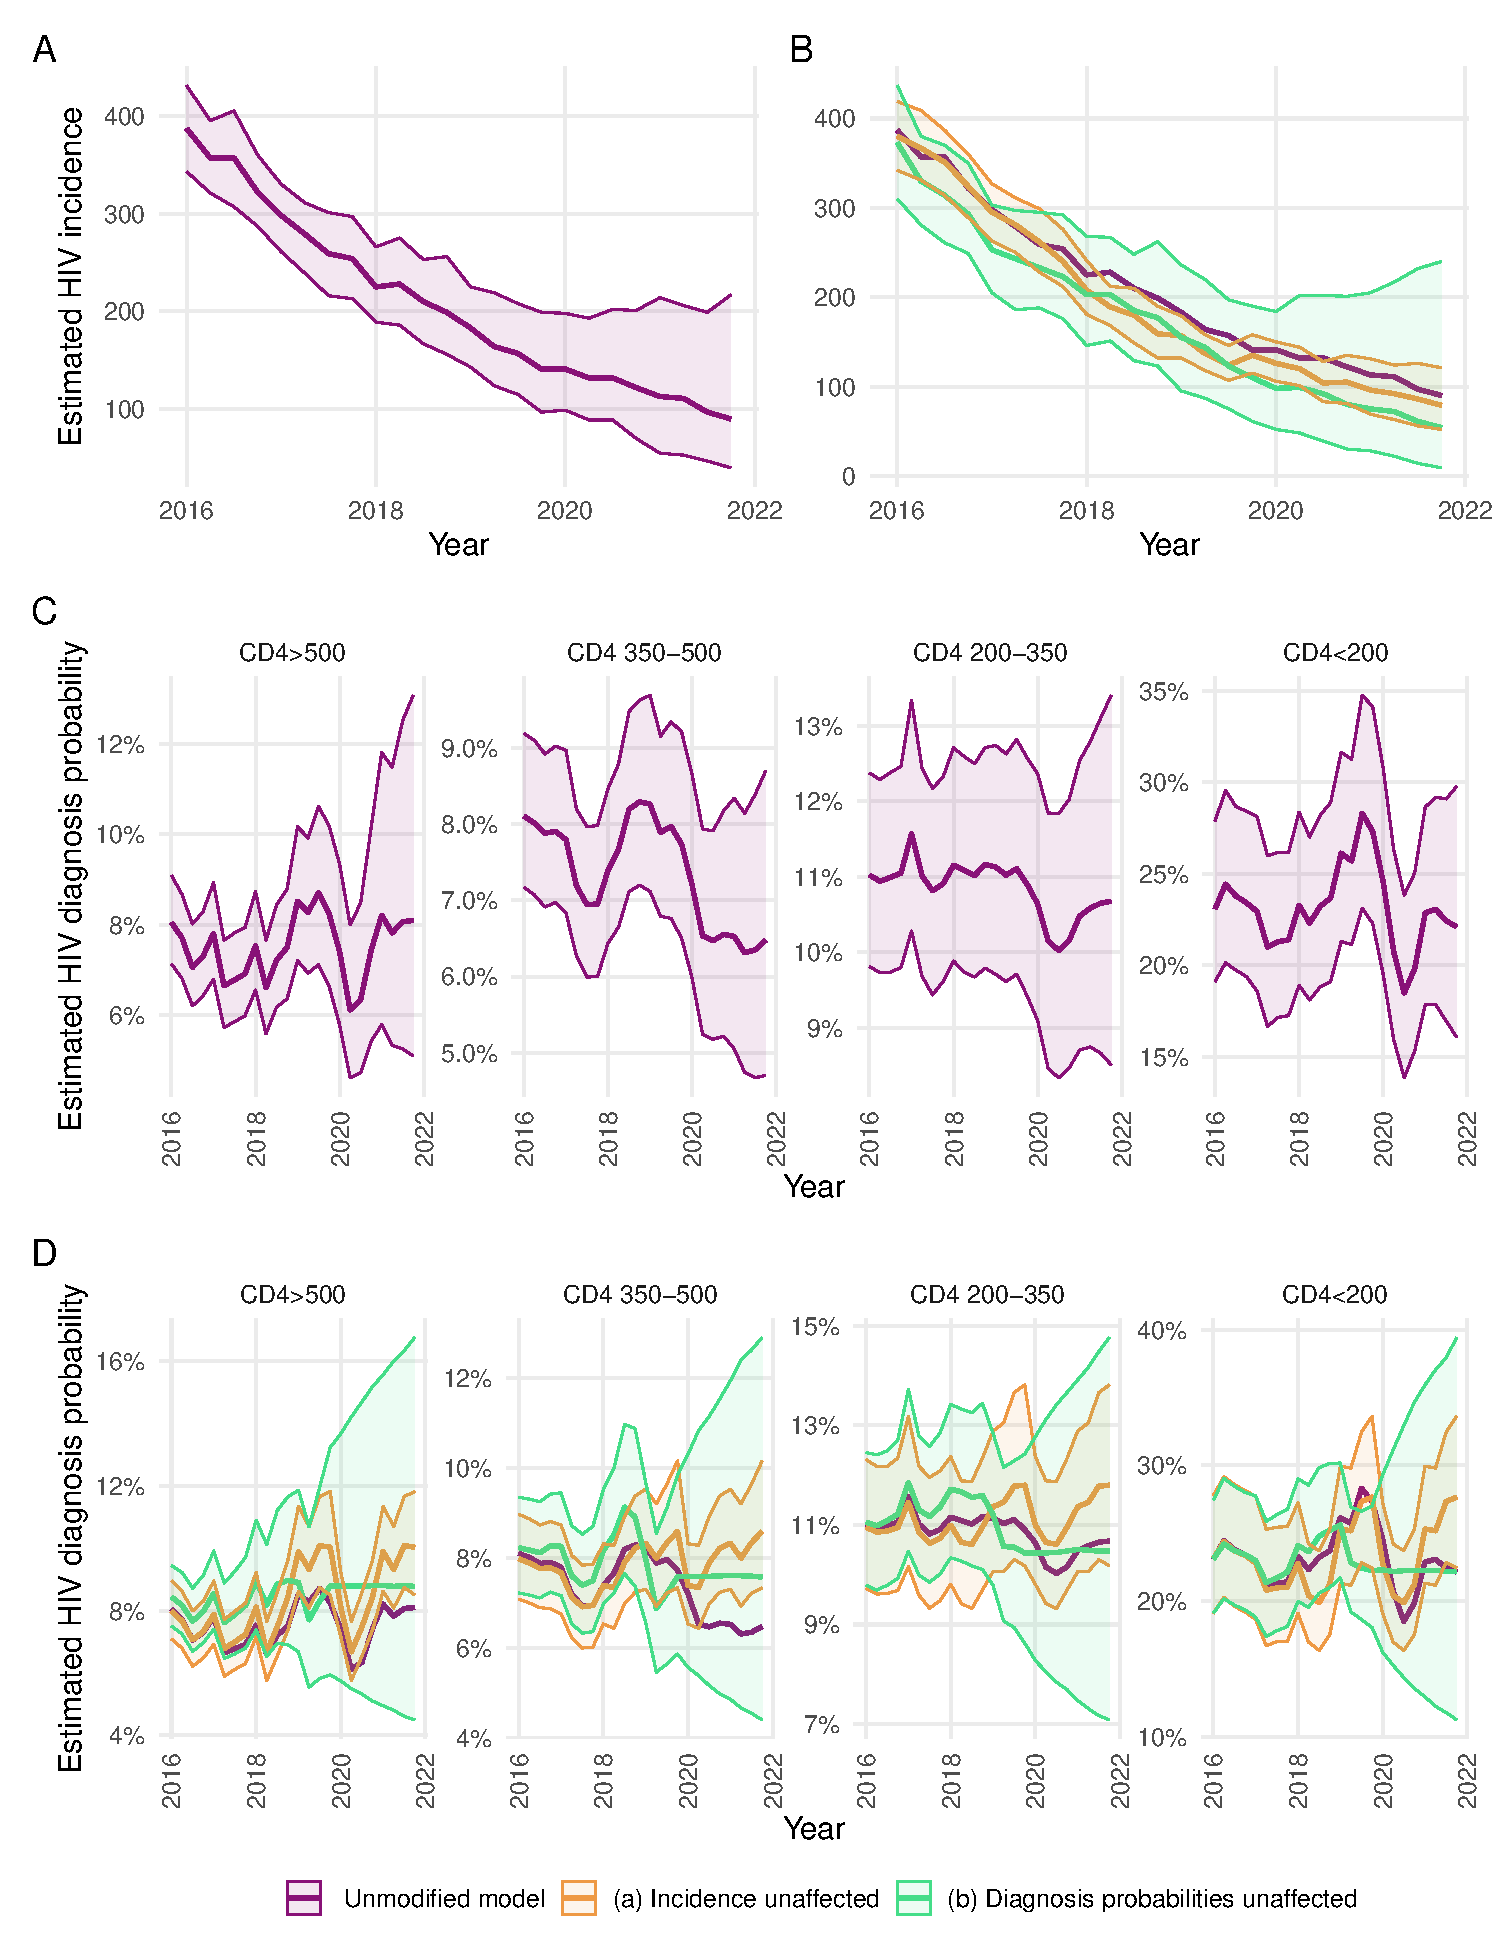
\includegraphics[width=\textwidth]{counterfactual_estimates.pdf}
  \caption[Estimated posterior median and 95\% CrI of HIV incidence and diagnosis probabilities fitted to HIV diagnosis data for GBM diagnosed in England, 2016--2021]{Estimated posterior median and 95\% CrI of HIV incidence (panels A and B) and diagnosis probabilities (panels C and D) fitted to HIV diagnosis data for GBM diagnosed in England, 2016--2021.}\label{fig:counterfactual_estimates}
\end{figure}

The posterior predictive estimates of HIV diagnoses in the unmodified model are shown in Figure~\ref{fig:counterfactual_fit} panel A, with corresponding estimates for scenarios (a) and (b) shown in panel B. The unmodified model had the closest fit to the data visually, whilst estimates for scenario (b) were less precise.

The LOOIC and the difference in the estimated log-likelihood between models is shown in Table~\ref{tab:hiv_looic}. Scenario (a) had the lowest LOOIC, although the difference in the log-likelihood between scenario (a) and the unmodified model was not significant. The LOOIC for scenario (b) was significantly higher than the other models indicating a poorer fit to the data.

\begin{figure}[htbp!]
  \centering
  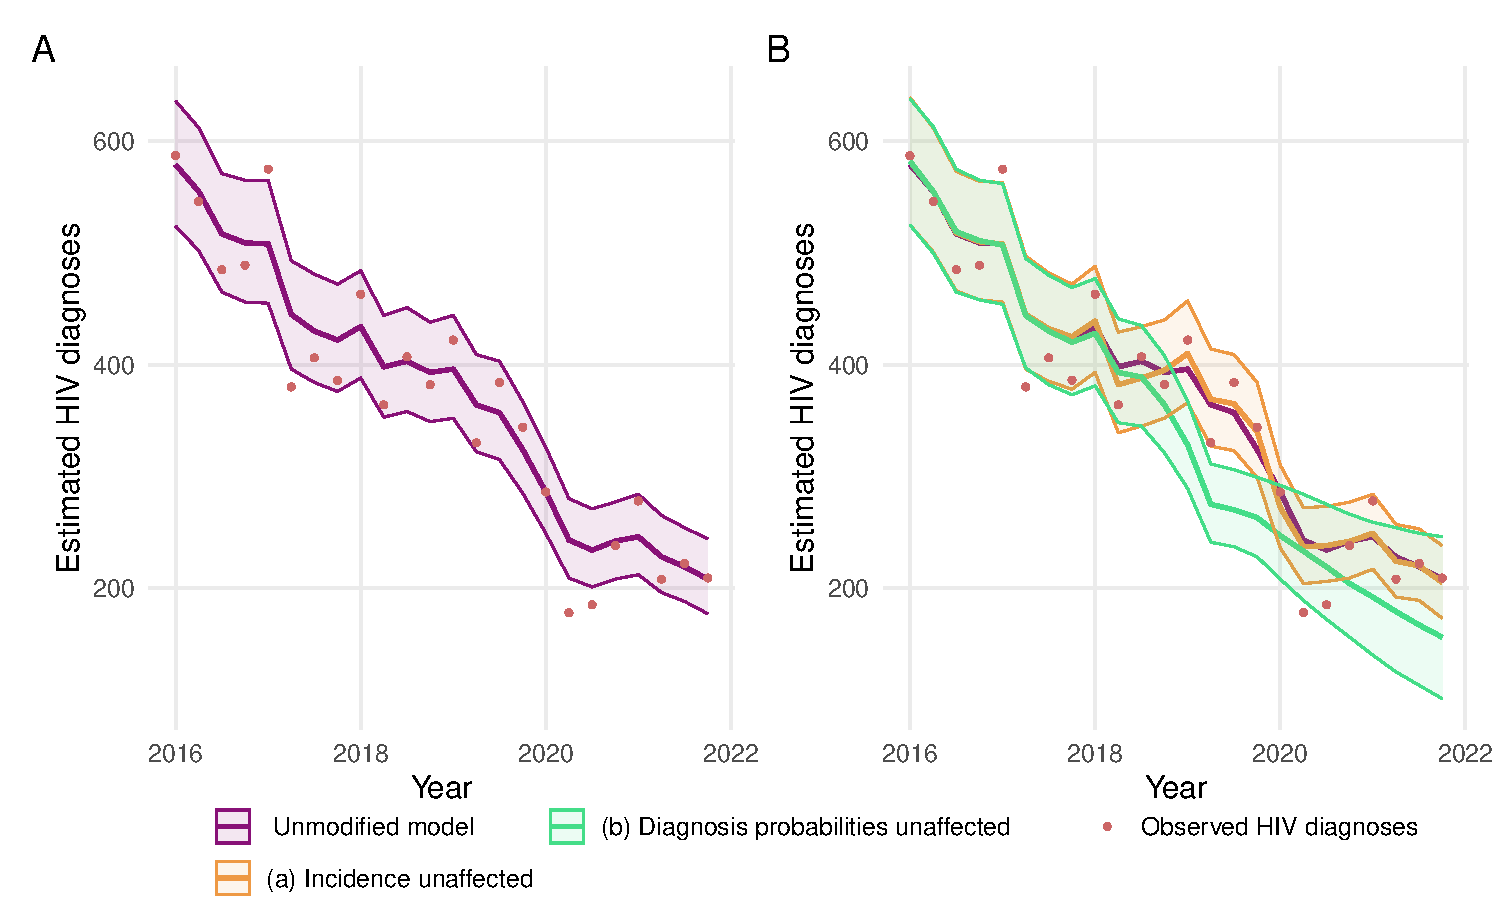
\includegraphics[width=\textwidth]{counterfactual_fit.pdf}
  \caption[Estimated HIV diagnoses (posterior predictive median and 95\% prediction interval), compared to observed HIV diagnosis data for GBM diagnosed in England, 2016--2021]{Estimated HIV diagnoses (posterior predictive median and 95\% prediction interval), compared to observed HIV diagnosis data for GBM diagnosed in England, 2016--2021.}\label{fig:counterfactual_fit}
\end{figure}

\begin{table}[!h]
\centering\centering
\caption{\label{tab:hiv_looic}LOOIC and difference in estimated log-liklihood values for unmodified model and each model scenario.}
\centering
\begin{tabular}[t]{lcc}
\toprule
 & LOOIC & \makecell[c]{Difference in estimated\\log-likelihood\\(Standard error)}\\
\midrule
Model scenario &  & \\
\hspace{1em}(a) Incidence unaffected & 4262.1 & 0 (0) \\
\hspace{1em}Unmodified model & 4269.8 & -3.8 (8.7) \\
\hspace{1em}(b) Diagnosis probabilities unaffected & 4495.7 & -116.8 (42.6) \\
\bottomrule
\end{tabular}
\end{table}


\subsection{Projected HIV incidence and progress towards HIV elimination targets}

\subsubsection{Methods}

Projected HIV incidence (to 2030) was previously estimated by~\cite{Brizzi2021-zl} using an age-dependent back-calculation model fitted to data to the end of 2018. These projections were re-run in light of the COVID-19 pandemic, using the CD4-only back-calculation model fitted to data to the end of 2022 (by which time HIV testing in SHS had largely returned to pre-pandemic levels~\parencite{Martin2023-um}).

To generate the projected incidence estimates, the incidence splines estimated by the back-calculation were extrapolated forwards using the \texttt{R} package \texttt{mgcv}~\parencite{Wood2016-ph}. Projected HIV incidence was compared to the previously published projections, and to the HIV Commission targets~\parencite{HIV_Commission2020-yy}. The proportion of extrapolated incidence profiles falling below the 250 and 50 thresholds were used to assess the likelihood of reaching the respective targets by 2025 and 2030.

\subsubsection{Results}

Projections of HIV incidence based on data to the end of 2018 are shown in Figure~\ref{fig:projected_incidence} panel A~\parencite{Brizzi2021-zl}, with updated projections based on data to the end of 2022 shown in panel B. Extrapolating forwards using the 2022 estimates, HIV incidence in 2025 was projected to be \var{est_hiv_2025} in 2025 and \var{est_hiv_2030} in 2030\@. Based on these projections, \var{prob_250_2022}\% of the extrapolated incidence profiles for 2025 were under 250, and \var{prob_50_2022}\% of those for 2030 were under 50.

\begin{figure}[htbp!]
  \centering
  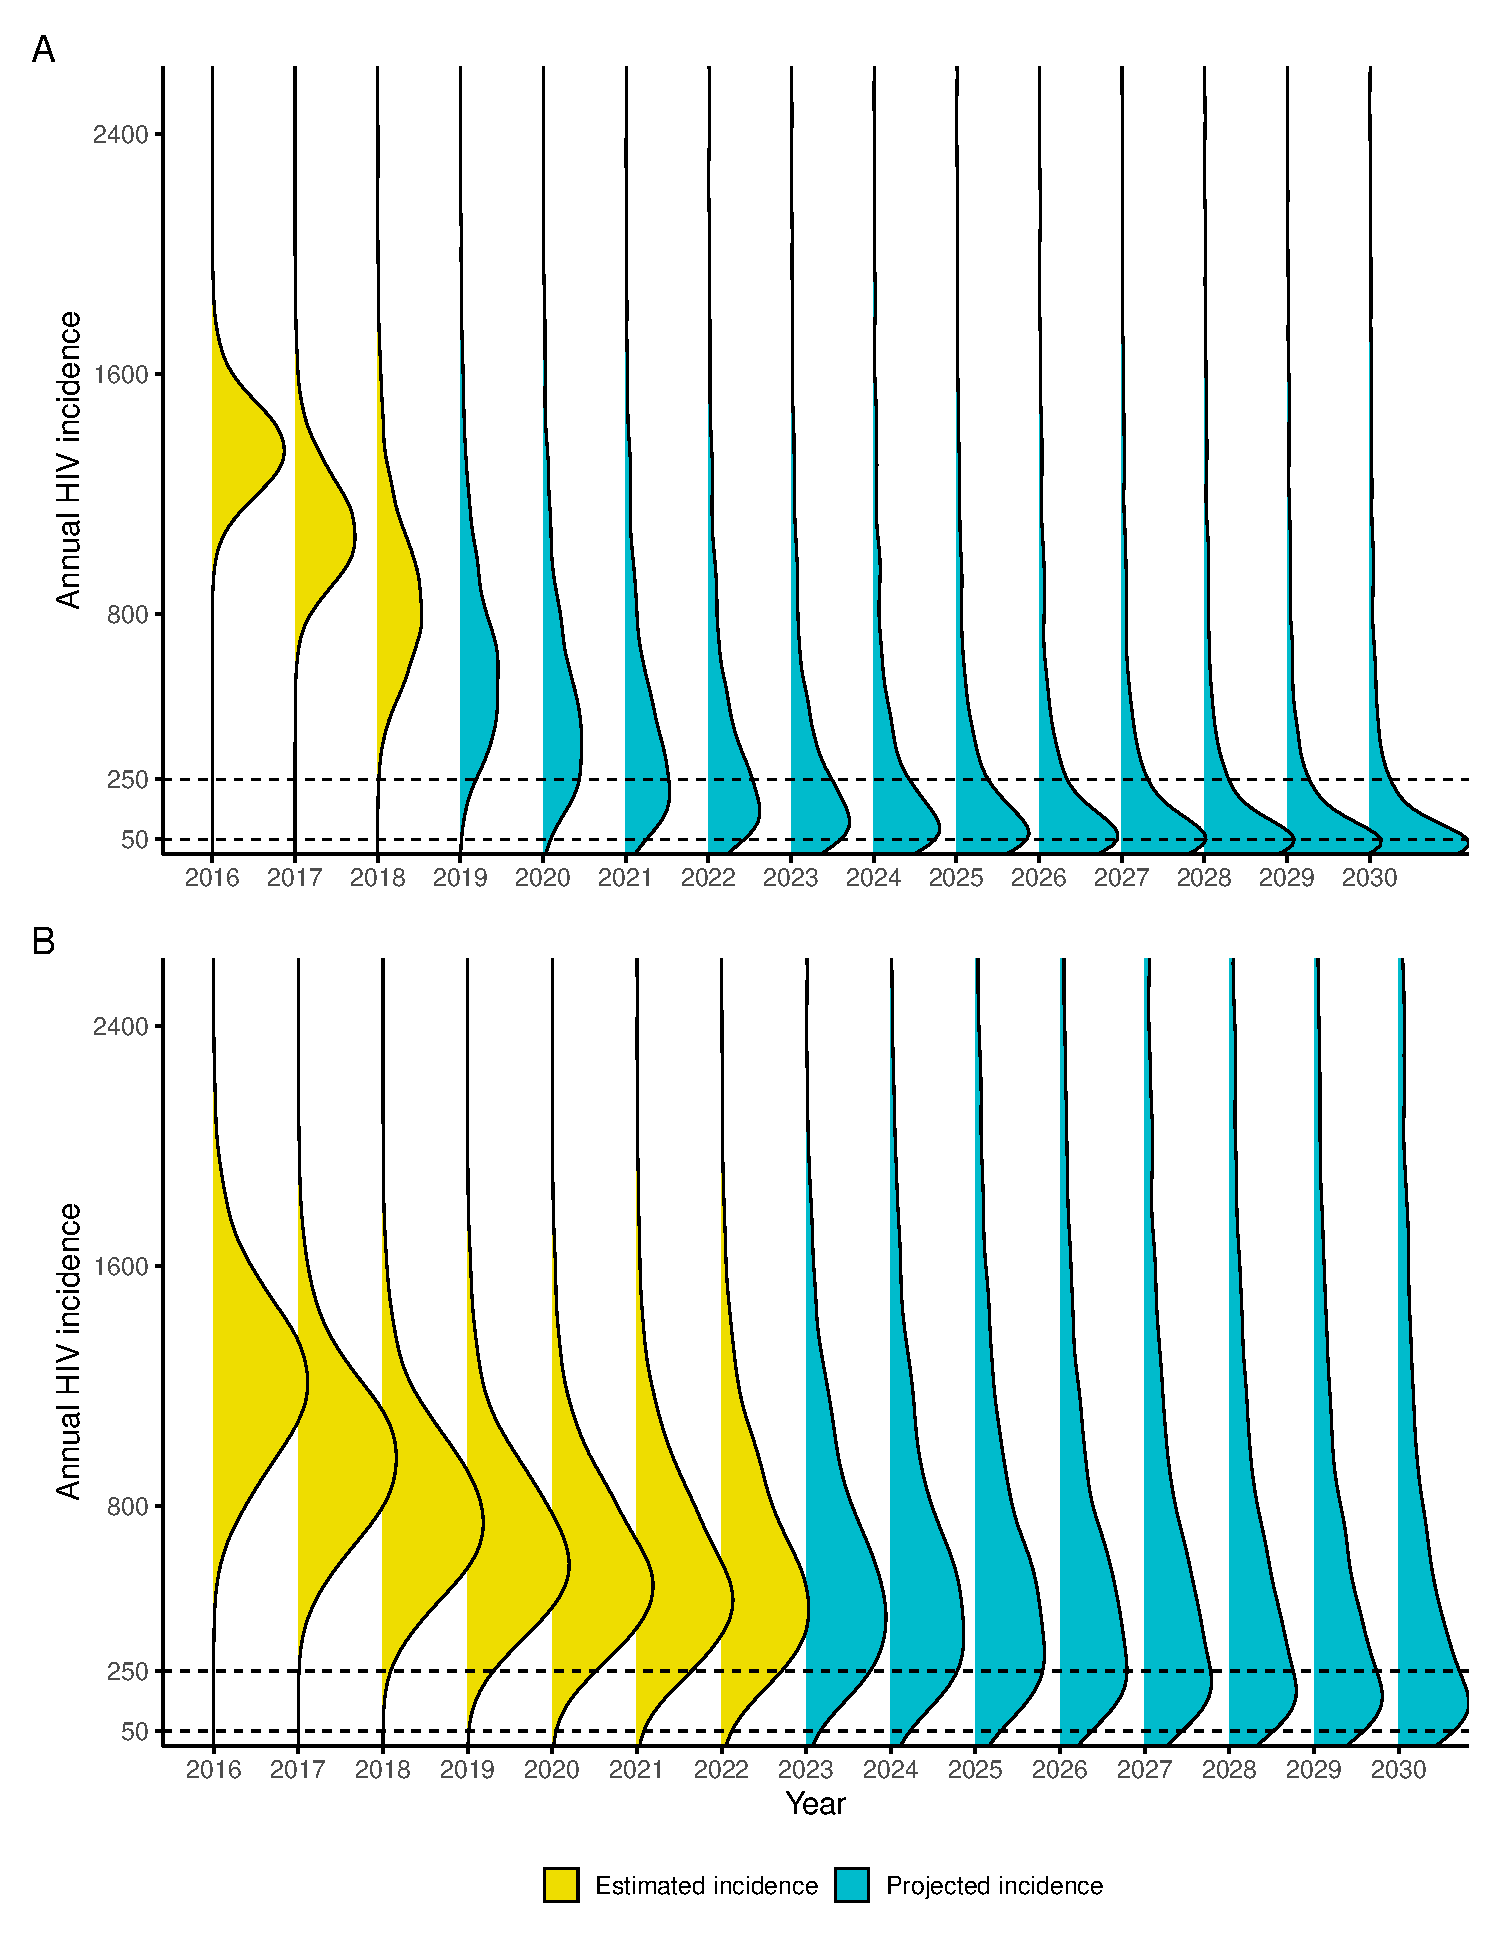
\includegraphics[width=\textwidth]{projected_incidence.pdf}
  \caption[Density plot of estimated and projected annual HIV incidence among GBM in England, 2016--2030]{Density plot of estimated and projected annual HIV incidence among GBM in England, 2016--2030, projections based on data to the end of 2018 (panel A), and data to the end of 2022 (panel B). Dotted lines indicate the HIV commission targets for HIV incidence among GBM of <250 by 2025, and <50 by 2030~\parencite{HIV_Commission2020-yy}.}\label{fig:projected_incidence}
\end{figure}

\subsection{Conclusions}

The COVID-19 lockdowns in 2020 and 2021 likely influenced both HIV transmission and testing activity. Two model scenarios with contrasting assumptions demonstrated that the back-calculation estimates were sensitive to the effect of lockdown being fixed entirely one way or the other. The results of these scenarios were included in UKHSA reports to show the potential impact of COVID-19 on HIV transmission in England~\parencite{Martin2022-iy}.

The best fitting model was scenario (a), in which HIV incidence was unaffected by COVID-19 lockdowns, but diagnosis probabilities were affected. In this scenario HIV diagnosis probabilities were estimated to have recovered by the end of 2020. Although the the reduction in HIV testing at sexual health services persisted beyond 2020, this may have been offset by the rapid expansion in self-sampling and home HIV testing, with around two thirds of HIV tests being accessed via internet services and conducted at home during the first national lockdown~\parencite{Wenlock2022-zk, Public_Health_England2020-qr}.

Although priors were specified differently for each scenario, all three models estimated a reduction in the posterior median for HIV incidence during 2020 and 2021. A continued reduction in incidence may be due to a combination of:\ lockdown, more widespread use of PrEP, a reduction in the number of condomless sex partners~\parencite{Pebody2021-fb}, and a high proportion of those living with HIV being unable to pass it on due to undetectable levels of virus~\parencite{World_Health_Organization2023-xi}.

A formal method of causal inference for a multi-state model is described in Chapter~\ref{cha:siren}, whereby elements of the transition matrix are fixed to pre-specified values to investigate the effectiveness of an intervention. The model scenarios presented in this section are not a formal causal analysis, but there are conceptual similarities:\ instead of fixing the elements of the transition matrices, strong prior information is placed on them, and the estimates corresponding to these different counterfactual scenarios are compared.

In previous projections, using data to the end of 2018, around 60\% of extrapolated incidence profiles reached the <250 target in 2025, and around 40\% reached the <50 target in 2030~\parencite{Brizzi2021-zl}. Projecting forwards from 2022 suggests that England is no longer on track to eliminate HIV transmission among GBM by 2030:\ under 17\% and under 5\% of extrapolated incidence profiles met the 2025 and 2030 targets, respectively. Estimates from the corresponding age-dependent model were more uncertain.

Whilst credible intervals overlap, the median projections for 2025 and 2030 from the back-calculation model are somewhat above those predicted by a simulation model which incorporates rates of testing, ART, and PrEP usage~\parencite{Cambiano2023-lj}. There is potential for future changes in HIV prevention and testing initiatives to accelerate the decline in HIV transmission, and progress towards the 2030 target should continue to be measured.

\subsubsection{Limitations}

Some lack of fit to the HIV diagnosis data was observed in all three models. Incorporating additional data sources, such as behavioural surveys and testing data around the time of lockdown, may help to to improve the precision and identifiability of these estimates.

As well as limiting the number of diagnoses occurring in 2020 and 2021, service disruption as a result of COVID-19 lockdowns may have led to under-reporting of new HIV diagnoses. UKHSA HIV surveillance teams cross-validate the HIV diagnosis data with an HIV commissioning database which collects service information among all people accessing care, and follow-up on individuals with missing diagnosis records. In the 2021 data archive, data quality was not considered to have been particularly affected by under-reporting as compared to the pre-COVID-19 pandemic period (C. Chau, personal communication).

As before, the back-calculation is not currently suitable for estimating HIV incidence as a result of heterosexual HIV transmission, and therefore not able to provide estimates of the impact of the COVID-19 pandemic on overall HIV incidence in England. A method utilising synthetically-controlled Bayesian structural time series to estimate the effect of COVID-19 lockdowns on HIV diagnoses has been applied to HIV diagnosis data for England and estimated a greater effect of COVID-19 lockdowns on diagnoses among GBM compared to heterosexual men and women~\parencite{Muhammed2024-dw}. There is substantial uncertainty in these estimates, however, and diagnosis data suggests a slowdown in the progress towards HIV elimination among heterosexual groups in particular~\parencite{Martin2023-um}.

\section{Chapter summary}

In this chapter I have developed the CD4 back-calculation model to incorporate additional biomarker information, and applied the resulting dual biomarker model to HIV surveillance data for GBM newly diagnosed in England. The dual biomarker model was shown to provide more precise estimates of HIV incidence, undiagnosed prevalence, and diagnosis probabilities compared to the CD4-only model. The new model also provided information about the probability of diagnosis in individuals with recently acquired HIV, which can be correlated with HIV prevention programmes for programme evaluation.

The sensitivity of the back-calculation to different assumptions about the effect of COVID-19 lockdowns in 2020 and 2021 was assessed, with the most likely scenario being a substantial reduction in the probability of diagnosis in 2020, with a swift recovery thereafter. Forward projections using data from the post-lockdown period suggest that England is no longer on track to eliminate HIV transmission among GBM by 2030, although this may not be only as a result of the pandemic.

At present the back-calculation model is only used for estimating HIV incidence among GBM, and not applied to other key prevention groups due to the assumption of no migration. The model also cannot be used to assess the specific impact of HIV prevention initiatives, such as PrEP, on HIV transmission. Further development to incorporate migration and transmission dynamics would enhance the utility and relevance of the model for all key prevention groups in England.
